\part{Wiskunde B}
\chapter{Differentiaalvergelijking}
\section{Definities}
De algemene definitie is:
$$F(x, y, y', y'', ..., y^{(n)}) = 0$$
waarbij: \begin{itemize}
\item \textbf{x} een veranderlijke is.
\item \textbf{y} een functie van x is.
\item er minstens één afgeleide van y is.
\end{itemize}
\example{Differentiaalvergelijking}{
    $$ x + y + y' = 0$$
}

Een differentiaalvergelijking heeft een \textbf{orde} en een \textbf{graad}
\begin{itemize}
    \item \textbf{Orde}: Dit is de orde van de hoogste afgeleide dat voorkomt, dus \textit{n}.
    \item \textbf{Graad}: De graad \textit{r} bestaat niet altijd maar is wel altijd een strik positief geheel getal. De graad is de macht die behoort tot de afgeleide met de grootste orde. $y^{(n)^{r}}$
\end{itemize}
\example{Orde en graad}{
    \begin{center}
        \begin{tabular}{l | l | l}
            Differentiaalvergelijking                          & Orde & Graad \\
            \hline
            $y\ - 2y'^3 = yx$                                  & 2    & 1     \\
            $1 + (y'')^4 + 2y' + x(y''')^2 = sin(x)$           & 3    & 2     \\
            $(x - 1)(y'') - xy' + y = 0$                       & 2    & 1     \\
            $e^s\frac{d^3s}{dt^3} + (\frac{ds^2}{dt^2})^3 = 0$ & 3    & 1     \\
            $xy' + e^{y'} + y'' = 1$                           & 1    & /     \\
            \hline
            $\sin\sqrt {y'} = x + 2$                           & 1    & /     \\
            $\;\;\rightarrow y' = \arcsin^2(x+2)$              & 1    & 1     \\
            \hline
            $\sin y' = xy'^2$                                  & 1    & /     \\
            $\;\;\rightarrow y' = \arcsin(xy'^2)$              & 1    & /     \\
            \hline
            $y^{'3} + \frac{x}{y''} + y'' = 1$                 & 2    & ?     \\
            $\;\;\rightarrow y^{'3}y'' + x + (y'')^2 = 1$      & 2    & 2     
            
        \end{tabular}
    \end{center}
}
\section{Soorten oplossingen}
Tijdens het oplossen van een differentiaalvergelijking van de \textit{n}-de orde worden drie oplossingen onderscheden:
\begin{enumerate}
\item De \textbf{Algemene oplossing (AO)}: Verzameling van functies zodat de differentiaalvergelijking klopt. De algemene oplossing bevat \textit{n }onafhankelijke constanten. Deze constanten zijn getallen en geen functies.
\item De \textbf{Particuliere oplossing (PO)}: Dit is één van de krommen van de AO en is afhankelijk van de beginvoorwaarden van het probleem.
\item De \textbf{Singuliere oplossing (SO)}: Een oplossing die niet voldoet aan de AO maar wel een oplossing is voor de DVG.
\end{enumerate}
\example{Onafhankelijke variabelen:}
{
\begin{center}
    \begin{tabular}{l | l | l}
    AO & Onafh. C & Orde DVG \\
    \hline
    $y = C_1 + C_2x$ & 2 & 2 \\
    $y = C_1  - C_1^2x$ & 1 & 1 \\
    \hline
    $y = C_1(C_2 + C_3e^x)$ & ? & ? \\
    $\;\;\rightarrow C_1C_2 + C_1C_3e^x$ & ? & ? \\
    $\;\;\rightarrow a + be^x$ & 2 & 2 \\
    \hline
    $y = C_1 + \ln(C_2 x)$ & ? & ? \\
    $\;\;\rightarrow y = C_1 + \ln(C_2) + \ln(x)$ & ? & ? \\
    $\;\;\rightarrow y = a + \ln(x)$ & 1 & 1


    \end{tabular}
\end{center}
}
\example{Oef 1 AO en PO}{Gegeven een differentiaalvergelijking: $y'' + y = 0$
\begin{enumerate}
\item Toon aan dat $y = a\sin(x) + b\cos(x)$ de AO is.
\item Geef enkele PO's.
\end{enumerate}
Oplossing:
\begin{enumerate}
\item 
\begin{equation*}
\begin{split}
    y & = a\sin(x) + b\cos(x) \\
    y' & = a\cos(x) - b\sin(x) \\
    y'' & = -a\sin(x) - b\cos(x) 
\end{split}
\end{equation*}
Hieruit volgt:
\begin{gather*}
    y'' + y  = 0 \\
    -a\sin(x) - b\cos(x) + \sin(x) + b\cos(x)  = 0  \\
    \rightarrow \hbox{Het is een oplossing}
\end{gather*}
De differentiaalvergelijking heeft orde 2. De y-vergelijking bevat 2 onafhankelijke constanten en de y-vergelijking is een oplossing. Hierdoor is y de AO van de differentiaalvergelijking.
\item Enkele PO's:
\begin{equation*}
\begin{split}
y & = 0\\
y & = \sqrt{2}\sin(x) \\
y & = \sin(x) + \cos(x)
\end{split}
\end{equation*}
\end{enumerate}
}

\example{Oef 2 AO en PO}
{Gegeven een differentiaalvergelijking: $y'^2 - yy'+e^x$
\begin{enumerate}
\item Geef de orde en graad.
\item Is $y = \frac{1}{C} + Ce^x$ de AO?
\item Wat  voor soort oplossing is $y = 2\sqrt{e^x}$
\end{enumerate}
Oplossing:
\begin{enumerate}
\item 
De orde is 1 en de graad is 2.

\item 
$$y' = Ce^x$$
\begin{equation*}
\begin{split}
\rightarrow C^2(e^x)^2 - (\frac{1}{C} + Ce^x)Ce^x + e^x &  = 0 \\
\Leftrightarrow C^2e^{2x} - e^x - C^2e^{2x} + e^x &  = 0 \\
\Leftrightarrow C^2e^{2x} - e^x - C^2e^{2x} + e^x & = 0 \\
\Leftrightarrow 0 & =0
\end{split}
\end{equation*}
$$\rightarrow \hbox{Het is een oplossing}$$
Orde DVG = 1 = Onafhankelijke constanten van y

\item 
$$ y'  = 2 \cdot \frac{1}{2\sqrt{e^x}} \cdot e^x = \sqrt{e^x}$$
\begin{equation*}
\begin{split}
\rightarrow & y'^2 - yy'+e^x \\
\Leftrightarrow &  (\sqrt{e^x})^2 - 2\sqrt{e^x}\cdot\sqrt{e^x} + e^x  = 0 \\
\Leftrightarrow & e^x - 2e^x + e^x  = 0 \\
\Leftrightarrow & 0 = 0
\end{split}
\end{equation*}
Dit is een singuliere oplossing aangezien y niet overeenkomt met de AO, maar wel voldoet aan de DVG.

\end{enumerate}
}
\section{Bepalen van een DVG}
Indien een AO gegeven is met \textit{n} onafhankelijke constanten:
\begin{enumerate}
\item Controleer of de constanten werkelijk onafhankelijk zijn.
\item Leid de AO \textit{n} maal af.
\item Elimineer de \textit{n} constanten van de \textit{n + 1} bekomen vergelijkingen. De laatste vergelijking moet zeker gebruikt worden.
\item Controleer of de DVG van orde \textit{n} is.
\end{enumerate}

\example{Oef 1 bepalen van een DVG}
{
De algemene oplossing is $$y = C_1 + C_2x$$
\begin{enumerate}
\item Er zijn \textit{2} onafhankelijke constanten.
\item Er moet \textit{2} keer afgeleid worden:
$$
    \begin{cases}
    y    & = C_1 + C_2x \\
    y'   & = C_2 \\
    y''  & = 0 \\
    \end{cases}
$$
\item De constanten zijn al geëlimineerd. 
\item De DVG is $y'' = 0$ en heeft orde \textit{2}.

\end{enumerate}
}

\example{Oef 2 bepalen van een DVG}
{
Bepaal de DVG van: $$y = C_1 + C_2e^{-x} + C_3e^{3x}$$
\begin{enumerate}
\item Er zijn \textit{3} onafhankelijke constanten.
\item Er moet \textit{3} maal afgeleid worden.
    \[ 
    \begin{cases}
            y & = C_1 + C_2e^{-x} + C_3e^{3x} \\
    y'     & = -C_2e^{-x} + 3C_3e^{3x}     \\
    y'' & = C_2e^{-x} + 9C_3e^{3x}      \\
    y''' & = -C_2e^{-x} + 27C_3e^{3x}
    \end{cases}
    \]

\item 
Tel de 1ste afgeleide op met de 2de afgeleide en tel de 2de afgeleide op met de 3rde afgeleide
\[
    \begin{cases}
    y + y''    & = 3C_3e^{3x} + 9C_3e^{3x} = 12C_3e^{3x}  \\
    y'' + y''' & = 9C_3e^{3x} + 27C_3e^{3x} = 36C_3e^{3x}
    \end{cases}
\]
Vermenigvuldig de 1ste vergelijking met 3 en trek hiervan de 2de vergelijking af.

$$3(y + y'') - y'' - y''' = 3(12C_3e^{3x}) - 36C_3e^{3x} = 0$$
$$\rightarrow y''' - 2y'' - 3y' = 0$$
\item
De orde van deze DVG is \textit{3}

\end{enumerate}
}

\example{Oef 3 bepalen van een DVG}
{
Bepaal de DVG van alle cirkels met middelpunt y = -x.
\begin{enumerate}
\item Eerst moet de AO gevonden worden. Het middelpunt van elke cirkel kan gegeven worden met $m(a, -a).$
    Hieruit volgt de algemene vergelijking van een cirkel: $$(x - a)^2 + (y + a)^2 = R^2$$
    Er zijn \textit{2} onafhankelijke constanten (a en R).
\item Er moet \textit{2} maal (impliciet) afgeleid worden.
\[
    \begin{cases}
    (x - a)^2 + (y + a)^2 = R^2 \\
    \frac{dy}{dx} : (x-a) + y'(y+a) = 0 \\
    \frac{d^2y}{dx^2} : 1 + y''(y + a) + y'^2 = 0
    \end{cases}
\]
\item
    Vorm $\frac{dy}{dx}$ om naar $a$:
    $$a = \frac{-x - yy'}{y' - 1}$$
    Substitueer deze $a$ in $\frac{d^2y}{dx^2}$:
    $$1 + y''(y + (\frac{-x - yy'}{y' - 1})) + y'^2 = 0$$
    $$\rightarrow 1 + y''(y + (\frac{x + yy'}{-y' + 1})) + y'^2 = 0$$
    $$\rightarrow y''(x + y) - y'^3 + y'^2 - y' + 1 = 0$$
\item Orde van de DVG = \textit{2}  = Aantal onafhankelijke constanten.
\end{enumerate}
}
\section{Oplossen van een lineaire DVG van orde n met constante reële coëfficiënten}
\begin{equation*}
 \begin{split}
		  & y''' - y''\sin t + ty = t^2 \\
  \Leftrightarrow & D^3y - D^2y\sin t + ty = t^2 \\
  \Leftrightarrow & (D^3 - D^2\sin t + t)y = t^2 \\
  \Leftrightarrow & L(d)y = g(t) \\
  \Leftrightarrow & \hbox{met} L(d) = \sum_{i = 0}^{n} a_iD^i \qquad ,a_i \in \mathbb{R}
 \end{split}
\end{equation*}
Een lineaire DVG is een DVG waarbij alle coëfficiënten van alle afgeleiden enkel voorkomen als eerste macht.
\subsection{Particuliere oplossing}
De particuliere oplossing kan slechts bepaald worden indien alle beginvoorwaarden 

($y(0), y'(0),...,y^{(n-1)}(0)$) gekend zijn.
\subsection{Algemene oplossing}
Indien de beginvoorwaarden niet gekend zijn moeten $y(0),y'(0)...y^{(n-1)}(0)$ respectievelijk gelijkgesteld worden aan $C_1, C_2, ..., C_n$

\example{
  Bepaal de PO van $y'' + y = g(t)$ indien $y(0) = 0$, $y'(0) = 1$ en 
  $$
    g(t) = \begin{cases}
	      0 & t < 1 \\
	      e^{-t} & t > 1
	   \end{cases}
  $$
}{
  \begin{equation*}
   \begin{split}
                   & L(d)y = g(t) \\
   \Leftrightarrow & (D^2 + 1)y = g(t) \\
   \Leftrightarrow & (D^2 + 1)y = e^{-t}H(t - 1) \\
   \mathcal{L}\{LL\}(s) & = \mathcal{L}\{y'' + y\}(s) \\
                        & = s^2Y - sy(0^{+}) + y'(0^{+}) + Y \\
                        & = s^2Y - 1 + Y \\
   \mathcal{L}\{RL\}(s) & = \mathcal{L}\{e^{-t}H(t - 1\}(s) \\
                        & = \mathcal{L}\{e^{-(t - 1) - 1}H(t - 1)\}(s) \\
                        & = e^{-1}\mathcal{L}\{e^{-(t - 1)}H(t - 1)\}(s) \\
                        & = e^{-1}e^{-s}\mathcal{L}\{e^{-t}\}(s) \\
                        & = e^{-1}e^{-s}\frac{1}{s + 1} \\
                        & = \frac{e^{-(s + 1)}}{s + 1} \\
   \hbox{dus} \\
   \Leftrightarrow & s^2Y - 1 + Y = \frac{e^{-(s + 1)}}{s + 1} \\
   \Leftrightarrow & Y(s^2 + 1) = 1 + \frac{e^{-(s + 1)}}{s+1} \\
   \Leftrightarrow & Y = \frac{1}{s^2 + 1} + \frac{e^{-(s+1)}}{(s+1)(s^2+1)}     \\
   \Leftrightarrow & \mathcal{L}^{-1}\{Y\}(t) = \mathcal{L}^{-1}\bigg\{\frac{1}{s^2 + 1} + \frac{e^{-(s+1)}}{(s+1)(s^2+1)}\bigg\}(t) \\
   \Leftrightarrow & y(t) = \sin t +e^{-1}f(t - 1)H(t - 1) \\
	   \hbox{met}\; f(t) & = \mathcal{L}^{-1}\bigg\{\frac{1}{(s + 1)(s^2 + 1)}\bigg\}(t) \\
			     & = \frac{1}{2}\mathcal{L}^{-1}\bigg\{\frac{1}{s + 1} - \frac{s - 2}{s^2 + 1}\bigg\}(t) \\
			     & = \frac{1}{2}\bigg[e^{-t} - (\cos t + \sin t)\bigg] \\
	    \hbox{antwoord: }\; y(t)  & = \sin t + \frac{1}{2}\bigg(e^{-t} - e^{-1}\cos (t - 1) + e^{-1} \sin (t - 1) \bigg)H(t - 1)
   \end{split}
  \end{equation*}

}
\example{
  Bepaal de PO van $y'' + y = \delta\big(t - \frac{\pi}{2}\big)$ indien $y(\frac{\pi}{4}) = 0$, $y'(\frac{\pi}{4}) = 0$
}{
  Stel: $y(0^+) = C_1$, $y'(0^+) = C_2$
  \begin{equation*}
   \begin{split}
    \mathcal{L}\{LL\}(s) & = \mathcal{L}\{y'' + y\}(s) \\
			 & = s^2Y - sC_1 - C_2 + Y \\
    \mathcal{L}\{RL\}(s) & = \mathcal{L}\bigg\{\delta\big(t - \frac{\pi}{4}\bigg)\bigg\}(s) \\
                         & = \int_0^{+\infty}\delta\big(t - \frac{\pi}{4}\big)e^{-st} \; dt \\
                         & = e^{-\frac{\pi}{2}s} \\
    \hbox{dus} \\
    \Leftrightarrow & s^2Y - sC_1 - C_2 + Y = e^{-\frac{\pi}{2}s}  \\
    \Leftrightarrow & Y = \frac{e^{-\frac{\pi}{2}s} + sC_1 + C_2}{s^2 + 1} \\
    \Leftrightarrow & \mathcal{L}^{-1}\{Y\}(t) = \mathcal{L}^{-1}\bigg\{\frac{e^{-\frac{\pi}{2}s} + sC_1 + C_2}{s^2 + 1}\bigg\}(t) \\
    \Leftrightarrow & y(t) = C_2\sin t + C_1\cos t + f\big(t - \frac{\pi}{2}\big)H\big(t - \frac{\pi}{2}\big)\\
    \hbox{met}\; f(t) & = \mathcal{L}^{-1}\bigg\{\frac{1}{s^2 + 1}\bigg\}(t) \\
                      & = \sin t\\
    \hbox{De algemene oplossing: }\; y(t)  & =  C_2\sin t + C_1\cos t - \bigg(\cos(t) H\big(t - \frac{\pi}{2}\big)\bigg)
   \end{split}
  \end{equation*}
  De PO voor $t = \frac{\pi}{4} \qquad ( < \frac{\pi}{2}\;\hbox{dus Heaviside is 0})$
  \begin{equation*}
   \begin{split}
    y(t) & = C_2 \sin t + C_1 \cos t  \Rightarrow y(\frac{\pi}{4})  : 0 = C_2\frac{\sqrt{2}}{2} + C_1\frac{\sqrt{2}}{2}\\
    y'(t) & = C_2 \cos t - C_1 \sin t \Rightarrow y'(\frac{\pi}{4}) : 0 = C_2\frac{\sqrt{2}}{2} - C_1\frac{\sqrt{2}}{2}\\
    & \begin{cases}
     0 = C_2 + C_1 \\
     0 = C_2 - C_1
    \end{cases} \Rightarrow C_2 = C_1 = 0
   \end{split}
  \end{equation*}
    Het antwoord:
    $$y(t) = -(\cos t)H(t - \frac{\pi}{2})$$
}
\section{DVG van de orde 1 en graad 1}
\subsection{Gescheiden veranderlijken}
Indien een DVG van orde 1 en graad 1 te schrijven is als
$$f(x)\;dx = g(y)\;dy$$
Algemeen:
\begin{equation*}
 \begin{split}
  M(x, y)\;dx & = -N(x, y)\; dy \\
  f(x)g(y)\;dx & = -h(x)i(y)\; dy \\
  \frac{f(x)}{h(x)}\; dx = & -\frac{i(y)}{g(y)}\;dy \\
  a(x) \; dx & = b(y)\; dy \\
  \int a(x) \; dx & = \int b(y) \; dy \\
  A(x) + C_1 & = B(y) + C_2 \\
  A(x) & = B(y) + C
 \end{split}
\end{equation*}
\example{
    Bepaal de AO van $yt + \sqrt{1 - t^2}y' = 0$
}{
    \begin{equation*}
     \begin{split}
      & yt\;dt + \sqrt{1 - t^2}\;dy = 0 \\
      \Leftrightarrow & \sqrt{1 - t^2}\;dy = -yt\;dt \\
      \Leftrightarrow & \frac{dy}{y}= -\frac{t\;dt}{\sqrt{1 - t^2}} \\
      \Leftrightarrow & \int \frac{dy}{y}= -\int \frac{t\;dt}{\sqrt{1 - t^2}} \\
      \Leftrightarrow & \ln |y| \sqrt{1 - x^2} + C \\
      \Leftrightarrow & y = e^{\sqrt{1 - x^2} + C} \\
      \Leftrightarrow & y = e^{\sqrt{1 - x^2}}e^C \\
      \Leftrightarrow & y = De^{\sqrt{1 - x^2}} \\
     \end{split}
    \end{equation*}

}

\todo{LES DINSDAG 13/03}
\section{Homogene DVG}
Een DVG is homogeen indien:
$$f(\lambda x, \lambda y) = \lambda^n f(x,y)$$
Indien een DVG homogeen is kan volgende oplossingsmethode toegepast worden:

\example{
        Bepaal de PO van : 
        $$\frac{dx}{dt} = \frac{x}{t(\ln t - \ln x)}$$
        waarvoor x(1) = 1.
}{
    Berekening algemene oplossing
    \begin{equation*}
     \begin{split}
      & \frac{dx}{dt} = \frac{x}{t(\ln t - \ln x)} \\
      \Rightarrow & t(\ln t - \ln x) \;dx - x\;dt = 0 \\
      \Rightarrow & t\ln\bigg(\frac{t}{x}\bigg)\;dx - x\;dt = 0 \\
      & \hbox{controle homogeen} \\
      \Rightarrow & \lambda t \ln\bigg(\frac{\lambda t}{\lambda x}\bigg) - \lambda x\\
      \Rightarrow & \lambda^1 (t \ln\bigg(\frac{t}{x}\bigg)  - x) \qquad \hbox{homogeen want M(x,t) en N(x,t) hebben } \lambda \hbox{ tot de eerste macht} \\
      & \hbox{substitutie } t = ux \\
      \Rightarrow & u \ln u \; dx - u \;dx + x\; du = 0 \\
      \Rightarrow & (u \ln u - u) \; dx = x \; du \\
      \Rightarrow & \int \frac{du}{u(\ln n -1)} = \int \frac{dx}{x} \\
      \Rightarrow & \ln | \ln u - 1| = \ln |x| + \ln |C| \\
      \Rightarrow & \ln | \ln u - 1| = \ln |Cx|  \\ 
      \Rightarrow & \ln u - 1 = Cx \\ 
      \Rightarrow & \ln u = Cx + 1 \\
      \Rightarrow & u = e^{Cx + 1} \\
      \Rightarrow & t = xe^{Cx + 1}
     \end{split}
    \end{equation*}
    Berekening particuliere oplossing:
    \begin{equation*}
     \begin{split}
      & x(1) = 1 \\
      \Rightarrow & 1 = 1e^{C + 1} \\
      \Rightarrow&  C + 1 = 0 \\
      \Rightarrow & C = -1 \\
      \Rightarrow & t = xe^{-x + 1}
     \end{split}
    \end{equation*}


}


\section{Exacte DVG}
\example{
    Bepaal alle functie f(y) zodanig dat de 
    DVG $$2y\; dx + (x - 4y\sqrt{y}) \; dy = 0$$
    na vermenigvuldiging met 
    f(y) exact wordt.Bepaal daarna haar AO.
}{
    Is deze DVG exact?
    \begin{equation*}
     \begin{split}
      \frac{\partial}{\partial y}2y & = 2 \\
      \frac{\partial}{\partial x}(x - 4y\sqrt{y}) & = 1
     \end{split}
    \end{equation*}
    Deze DVG is dus niet exact. We moeten een functie f(y) bepalen zodat deze DVG wel exact wordt.
    $$2yf(y)\; dy + (x - 4y\sqrt{y})f(y)\; dy = 0$$
   \begin{equation*}
    \begin{split}
     & \partialof{y}2yf(y)  = \partialof{x}(x - 4y^{3/2}) f(y) \\
     \Rightarrow & 2f(y) + 2y\derivativeof{y}f(y)  = f(y) \\
     \Rightarrow &  2y \derivativeof{y}f(y)  = -f(y) \\
     \Rightarrow & \frac{d}{f(y)}f(y) = - \frac{dy}{2y} \\
     \Rightarrow & \int \frac{d}{f(y)}f(y) = - \int  \frac{dy}{2y} \\
     \Rightarrow & \ln|f(y)| = -\frac{1}{2}\ln|y| + \ln|C| \\
     \Rightarrow & \ln|f(y)| = -\frac{1}{2}\ln|Cy| \\
     \Rightarrow & \ln|f(y)| = \ln|Cy|^{-1/2} \\ 
     \Rightarrow & f(y) = \frac{1}{\sqrt{Cy}} \\
     \Rightarrow & f(y) = \frac{1}{\sqrt{y}} \qquad \hbox{met C = 1}
    \end{split}
   \end{equation*}
   De DVG wordt:
   $$2\sqrt{y}\; dx  + \bigg(\frac{x}{\sqrt{y}} - 4y\bigg)\; dy = 0$$
   wat een een exacte DVG oplevert. Nu bepalen we de AO.
   \begin{equation*}
    \begin{split}
     & 2\sqrt{y}\; dx  + \bigg(\frac{x}{\sqrt{y}} - 4y\bigg)\; dy = 0 \\
     &   \hbox{komt overeen met} \\
     & \partialof{x}F\; dx + \partialof{y}F\;dy = 0
    \end{split}
   \end{equation*}
    We krijgen volgend stelsel:
    $$\begin{cases}
       \partialof{x}F = 2\sqrt{y} (*) \\
       \partialof{y}F = \frac{x}{\sqrt{y}} - 4y (**)
      \end{cases}
    $$
    \begin{equation*}
     \begin{split}
      (*) & \partialof{x}F = 2\sqrt{y}  \\
      \Rightarrow & F = \int 2\sqrt{y}\; dx  \\
      \Rightarrow & F = 2\sqrt{y}x + h(y); \\
      (**) & \partialof{y} = \frac{x}{\sqrt{y}} - 4y = 2x\frac{1}{2\sqrt{y}} + \derivativeof{y}h(y) \\
      \Rightarrow & \derivativeof{y}h(y) = -4y \\
      \Rightarrow & h(y) = \int -4y \; dy \\
      \Rightarrow & h(y) = -2y^2
     \end{split}
    \end{equation*}
    De AO:
    $$F(x, y) = 2\sqrt{y}x - 2y^2$$
}
\example{
    In een vat bevindt zich $20 m^3 $
zout-oplossing waarin 1 kg zout opgelost is. Men voert een nieuwe pekeloplossing toe met 
constante concentratie van 0,5 kg zout/$m^3$
en aan een snelheid 
van $2m^3$/min. De oplossing wordt continu gemengd en loopt onderaan weg met een snelheid van $1m^3$/min. 
Hoeveel zout bevindt zich in de pekeloplossing na 1 uur?
}{
    Definitie van de variabelen:
    \begin{itemize}
     \item $x : \#$ kg zout na $t$ minuten
     \item Op $t = 0$ is $x(0) = 1$
     \item $C_i = \frac{1}{2}kg/m^3$ (Concentratie in)
     \item $v_i = 2m^3/min$          (Snelheid in) 
     \item $C_{uit} = \frac{x(t)}{v(t)}$ (Concentratie uit)
     \item $v_{uit} = 1m^3/min$     (Snelheid uit)
    \end{itemize}
    We zoeken een uitdrukking voor $dx$.
    \begin{itemize}
     \item $dx = $ verandering $x$ gedurende $dt$ minuten
     \item $dx = $ hoeveelheid zout binnen gedurende $dt$ minuten - hoeveelheid zout buiten gedurende $dt$ minuten
    \end{itemize}
    Berekening AO:
    \begin{equation*}
     \begin{split}
      & dx = C_iv_i \; dt - C_{uit}v_{uit} \; dt \\
      \Rightarrow & dx = \frac{1}{2}\cdot 2\; dt - \frac{x(t)}{V(t)}\cdot 1\; dt \qquad \hbox{met } V(t) = 20 + 2t - t = 20 + t\\
      \Rightarrow & dx = dt - \frac{x}{20 + t} \; dt \\
      \Rightarrow & dx + \bigg(\frac{x}{20 + t} - 1\bigg)\;dt = 0 \\
      \Rightarrow & (20 + t)\;dx + (x - 20 - t)\;dt = 0 \\
       & \partialof{t}(20 + t) = 1 = \partialof{x}(x - 20 - t) \Rightarrow \hbox{exact} \\
       & \begin{cases}
        \partialof{x}F = 20 + t (*) \\
        \partialof{t}F = x - 20 -t (**)
       \end{cases} \\
       (*) & \partialof{x}F = 20 + t \\
        \Rightarrow & F = \int( x- 20 - t)\; dt \\
                    & = xt - 20t - \frac{t^2}{2} + h(x) \\
        \Rightarrow & 20 + t = \partialof{x}(xt - 20t - \frac{t^2}{2} + h(x)) \\
        \Rightarrow & 20 +t = t + \partialof{x}h(x) \\
        \Rightarrow & \derivativeof{x}h(x) = 20 \\
        \Rightarrow & h(x) = \int 20\;dx = 20x \\
        \Rightarrow & F = xt - 20t - \frac{t^2}{2} + 20x \\
        & \hbox{AO: } xt - 20t - \frac{t^2}{2} + 20x = C
     \end{split}
    \end{equation*}
    Bereken PO. Indien $x(0) = 1$ dan $C = 20$. 1 uur = 60 minuten $\Rightarrow$ x(60)
    \begin{equation*}
     \begin{split}
      & xt + 20x = 20t + \frac{t^2}{2} + 20 \\
      \Rightarrow & x = \frac{20t + \frac{t^2}{2} + 20}{20 + t} \\
      \Rightarrow & x(60) = 37.75\; kg
     \end{split}
    \end{equation*}

    
}


\section{Lineaire DVG van orde 1}
Algemene definitie:
$$\hbox{Een DVG is lineair in y en y' indien } y' + P(x)y = Q(x)$$
\example{ 
    $$dy + (y\sin x - \cos x)\; dx = 0$$
}{
    \begin{equation*}
     \begin{split}
      & dy + (y\sin x - \cos x)\; dx = 0 \\
      \Rightarrow & \frac{dy}{dx} + y\sin x - \cos x = 0 \\
      \Rightarrow & y' + y\sin x = \cos x
     \end{split}
    \end{equation*}
    Lineair in y en y'
}
\example{ 
    $$ds + (1 - 2t)s\;dt = t^2\;dt$$
}{
    \begin{equation*}
     \begin{split}
      & ds + (1 - 2t)s\;dt = t^2\;dt \\
      \Rightarrow & \frac{ds}{dt} + (1 - 2t)s = t^2
     \end{split}
    \end{equation*}
    Lineair in s en s'
}
\subsection{Oplossingsmethode}
\begin{equation*}
 \begin{split}
  & y' + P(x)y = Q(x) \\
  & \hbox{substitutie y = uv} \qquad \hbox{(vrijheidsgraad toevoegen)}\\
  \Rightarrow & u'v + uv' + P(x)uv = Q(x) \\
  \Rightarrow & u(P(x) + v') + u'v = Q(x) \qquad (*) \\
  & \hbox{stel P(x) + v' = 0 (vrijheidsgraad wegnemen)} \\
  \hbox{Bijgevolg: } \Rightarrow & \frac{dv}{dx} = - P(x)v \\
    \Rightarrow & \int \frac{dv}{v} = - \int P(x)\; dx \\
    \Rightarrow & \ln|v| = - \int P(x)\; dx \\
    \Rightarrow & v  = e^{-\int P(x)\; dx} \\
    (*)\Rightarrow & \frac{du}{dx} = \frac{Q(x)}{v} \\
    \Rightarrow & du = e^{\int P(x)\;dx}Q(x) \; dx \\
    \Rightarrow & u = \int e^{\int P(x)\;dx}Q(x) \; dx \\
    & \hbox{Vervang substitie om AO te bekomen}
 \end{split}
\end{equation*}

\example{
    Bepaal de AO van
    $$(4r^2s - 6)\; dr + r^3 \; ds = 0$$
}{
    \begin{equation*}
     \begin{split}
      & r^3\frac{ds}{dr} + 4r^2s - 6 = 0 \\
      \Rightarrow & \frac{ds}{dr} + \frac{4}{r}s = \frac{6}{r^3} \\
      \Rightarrow & s' + P(r)s = Q(r) \\
      & \hbox{substitutie s = uv} \\
      \Rightarrow & u'v + uv' + \frac{4}{r}uv = \frac{6}{r^3} \\
      \Rightarrow & u\bigg(v' + \frac{4}{r}v\bigg) + u'v = \frac{6}{r^3} \\
       & \frac{dv}{dr} = -\frac{4}{r}v \\
       & \int \frac{dv}{v} = -4\int \frac{dr}{r} \\
       & \ln |v| = -4 \ln |r| \\
       & v = r^{-4} \\
       \Rightarrow & \frac{du}{dr}\cdot\frac{1}{r^4} = \frac{6}{r^3} \\
       \Rightarrow & \frac{du}{dr}\cdot\frac{1}{r} = 6 \\
       \Rightarrow & \int du = \int 6r\; dr \\
       \Rightarrow &  u = 3r^2 + C \\
        & s = uv = (3r^2 + C)\frac{1}{r^4} \\
        & s = \frac{3}{r^2} + \frac{C}{r^4} \qquad \forall C \in \mathbb{R}
     \end{split}
    \end{equation*}

}

\section{DVG van type Bernouilli}
Een DVG is van type Bernouilli indien
$$y' + P(x)y = Q(x)y^n \qquad \hbox{met } n \in \mathbb{R}$$
\subsection{Oplossingsmethode}
Bewijs:
$$\frac{y'}{y^n} + P(x)\frac{y}{y^n} = Q(x)$$
Substitutie: $$z = \frac{y}{y^n} = y^{1 - n}$$
Waaruit volgt: $$z' = \frac{dz}{dx} = \frac{dz}{dy}\frac{dy}{dz}$$
\begin{equation*}
 \begin{split}
  z' & = (1 - n)y^{1 - n - 1}y' \\
     & = (1 - n)y^{-n}y' \\
     & = \frac{(1 - n)y'}{y^n}
 \end{split}
\end{equation*}
De DVG wordt:
$$\frac{z'}{1 - n} + P(x)z = Q(x)$$
Of beter geschreven:
$$z' + (1 -n)P(x)z = (1 - n)Q(x)$$
De DVG is lineair in z en z'

\example{
    Bepaal de AO vanaf $$xy\;dx = (x^2 - y^4) \;dy$$
}{
    \begin{equation*}
     \begin{split}
      & xy \; dx + (y^4 - x^2)\;dy = 0 \\
      \Rightarrow & xy \frac{dx}{dy} + (y^4 - x^2) = 0 \\
      \Rightarrow & \frac{dx}{dy} + \frac{y^4 - x^2}{xy} = 0 \\
      \Rightarrow & \frac{dx}{dy} - \frac{x}{y} + \frac{y^3}{x} = 0 \\
      \Rightarrow & \frac{dx}{dy} - \frac{1}{y}x = -y^3\frac{1}{x} 
     \end{split}
    \end{equation*}
    Bernouilli in x en x'
    $$      \Rightarrow  x\frac{dx}{dy} - \frac{1}{y}x^2 = -y^3$$
    stel $z = x^2$ dus $z' = 2x\frac{dx}{dy}$ 
    \begin{equation*}
     \begin{split}
      & \frac{1}{2}\frac{dz}{dy} - \frac{1}{y}z = -y^3 \\
      \Rightarrow & \frac{dz}{dy} - \frac{2z}{y} = -2y^3 \\
      & \hbox{substitutie } z = uv \\
      \Rightarrow & u'v + uv' - \frac{2uv}{y} = -2y^3 \\
      \Rightarrow & u(v' - \frac{2v}{y}) + u'v = -2y^3 \\ 
      & \frac{dv}{dy} = \frac{2v}{y} \\
      & \int \frac{dv}{v} = 2 \int \frac {dy}{y} \\
      & \ln |v| = 2\ln |y| \\
      & v = y^2  \\
      \Rightarrow&  \frac{du}{dy}y^2 = -2y^3 \\
      \Rightarrow & \int \frac{du}{dy} = - \int 2y \; dy \\
      \Rightarrow & u = -y^2 + C
     \end{split}
    \end{equation*}
    $z = x^2$ en $z = uv = y^2(C - y^2)$
    De AO wordt:
    $$x^2 + y^4 = Cy^2$$


}


\section{Orthogonale krommenbundel}
Definitie: elke kromme uit de ene bundel snijdt elke kromme uit de andere bundel loodrecht.
$$
    \begin{cases}
     f(x, y, C) = 0 \\
     f_{\bot}(x, y, C) = 0
    \end{cases}
$$
Raaklijn van $f$ staat loodrecht op raaklijn van $f_{\bot}$. Wiskundig wordt dit vertaald door: $\omega_{RL_{\bot}} = -\frac{1}{\omega_{RL}} = -\frac{1}{y'}$
De DVG van de orthogonale krommenbundel is
$$F_{\bot}\bigg(x, y, -\frac{1}{y'}\bigg)$$
\example{
    Bepaal de DVG van de orthogonale krommenbundel van alle raaklijnen aan $y = x^2$.
}{
    Elk punt op parabool kan beschreven worden als $p(a, a^2)$.
    \begin{enumerate}
     \item De vergelijking van de originele krommenbundel
        \begin{equation*}
         \begin{split}
          & y - a^2 = 2a(x - a) \\
          \Rightarrow & y - a^2 = 2ax - 2a^2 \\
          \Rightarrow & y = 2ax - a^2
         \end{split}
        \end{equation*}
     \item DVG van de originele krommenbundel
        $$
            \begin{cases}
             y = 2ax - a^2 \\
             y' = 2a
            \end{cases} \Rightarrow
            y = y'x - \frac{y'^2}{4}
        $$
     \item DVG van de orthogonale krommenbundel
        $y' wordt -\frac{1}{y'}$
        $$ y = \frac{1}{y'}x - \frac{1}{4}\frac{1}{y'^2}$$
        Uiteindelijk:
        $$4y'^2y = -4xy' - 1$$
    \end{enumerate}
    Deze DVG heeft graad 2, wat niet in deze cursus besproken wordt. Het is dus onoplosbaar.

}
\example{
    Bepaal de orthogonale krommenbundel van alle parabolen met top in de oorsprong en symmetrieas de X-as.
}{
    \begin{enumerate}
     \item De vergelijking van de originele krommenbundel
            $$ x = Cy^2$$
     \item DVG van de originele krommenbundel. Er is 1 onafhankelijke constanten dus 1 keer afleiden
            $$
              \begin{cases}
               x = Cy^2 \\
               1 = 2Cyy'
              \end{cases}
            $$
            Hieruit volgt $C = \frac{x}{y^2}$ en dus $1 = \frac{2xy'}{x}$
     \item DVG van de orthogonale krommenbundel
            
            $y'$ vervangen door $-\frac{1}{y'}$ dus
            $$1 = -\frac{2x}{yy'} \Leftrightarrow yy' = -2x$$
     \item DVG oplossen
     \begin{equation*}
      \begin{split}
                    & y \frac{dy}
                             {dx} = -2x \\
                    & \int y \; dy = - \int 2x\; dx \\
                    & \frac{y^2}{2} = -x^2 \\
                    & \frac{y^2}{2} + x^2 = C
      \end{split}
     \end{equation*}
     Dit zijn dus ellipsen

    \end{enumerate}


}
\section{DVG van hogere orde}
\example{
    Los op
    $$y''' = e^{-2x}$$
}{
    \begin{equation*}
     \begin{split}
       y''' & = e^{-2x} \\
       y''  & = \int e^{-2x}\;dx = -\frac{1}{2}e^{-2x} + C_1 \\
       y'   & = -\int \frac{1}{2}e^{-2x} + C_1 \; dx \frac{1}{4}e^{-2x} + C_1x + C_2 \\
       y    & = -\frac{1}{8}e^{-2x} + \frac{C_1x^2}{2} + C_2x + C_3 \\
            & = -\frac{1}{8}e^{-2x} + C_1x^2 + C_2x + C_3
     \end{split}
    \end{equation*}
}
\subsection{DVG van orde 2 van type F(x, y', y'') = 0}
Bewijs oplossingsmethode:

Stel $y' = p$, dan wordt $y'' = \frac{dp}{dx}$. De differentiaalvergelijking wordt $F(x, p, \frac{dp}{dx} = 0$. Dit is een dvg van orde 1 in p en x. 

\example{
    Bepaal de AO van $xy'' = y' - x$
}{
    $xy'' = y' - x $ komt overeen met $F(x , y', y'')$
    
    Stel $y' = p' \rightarrow y'' = x\frac{dp}{dx} = p - x$ waaruit volgt dat $x\;dp = (p - x)\;dx$. Dit is homogeen ($\lambda^{(1)}$ dus we stellen $p = ux$
    \begin{equation*}
     \begin{split}
      x(u\;dx + x\;du) & = (ux - x)\;dx \\
      u\;dx + x\;du    & = (u - 1) \;dx \\
      x\;du            & = -dx; \\
      du               & = -\frac{dx}{x} \\
      \int du          & = -\int\frac{dx}{x} \\
      u                & = \ln|x| + C_1 \\
      \frac{dy}{dx}    & = -x\ln|x| + C_1x \\
      \int dy          & = -\int x\ln|x| + C_1x \;dx
     \end{split}
    \end{equation*}
    Het Antwoord is:
    $$y = \frac{-x^2}{2}\ln|x| + \frac{x^4}{4} - C_2 + \frac{C_1}{2}x^2 = \frac{-x^2}{2}\ln|x| + \frac{x^4}{4} - C_2 + C_1x^2$$
}
\subsection{DVG van orde 2 van type F(y, y', y'') = 0}
Bewijs oplossingsmethode:

Stel $y' = p$, dan wordt $y'' = \frac{dp}{dx} = \frac{dp/dy}{dx/dy} = \frac{dp}{dy}\frac{dy}{dx} = p\frac{dp}{dy}$. De differentiaalvergelijking wordt $F(y, p, p\frac{dp}{dx} = 0$. Dit is een dvg van orde 1 in p en y.

\example{
    Bepaal de PO van $(1 - y)^2y'' - y'^3 = 0$ met $y(0) = 2$ en $y'(0) = 1$
}{
    Stel $y' = p \rightarrow y'' = p\frac{dp}{dy}$
    \begin{equation*}
     \begin{split}
      (1 - y)^2p\frac{dp}{dy} - p^3 & = 0 \\
      (1 - y)^2\frac{dp}{dy} - p^2  & = 0 \\
      (1 - y)^2\frac{dp}{dy}        & = p^2 \\
      \frac{dp}{p^2}                & = \frac{dy}{(1 - y)^2} \\
      \int \frac{dp}{p^2}           & = \int\frac{dy}{(1 - y)^2} \\
      -\frac{1}{p}                  & = -\frac{1}{1 - y} + C_1 \\
      C_1 & = 0 \quad \hbox{aangezien p(0) = 1 en y(0) = 2} \\
      \frac{1}{p} = \frac{dx}{dy} & = \frac{1}{y - 1} \\
      & \begin{cases}
       dx = \frac{dy}{y - 1} \\
       x = \ln|y - 1| + C_2 \\
       0 = \ln|1| + C_2 \rightarrow C_2 = 0
      \end{cases} \\
      x & = \ln|y - 1| \\
      e^x & = y - 1 \\
      y & = e^x + 1 
     \end{split}
    \end{equation*}

}
\section{Stellingen voor lineaire differentiaalvergelijkingen}
Voor geen enkele stelling is het bewijs te kennen
\subsection{Stelling 1}
Is $L(D)y = 0$ een lineaire homogene DVG van $n^{de}$ orde en $y_i(x), i = 1, ..., n$ n onafhankelijke PO's van $L(D)y = 0$ dan is $y = C_1y_1(x) + C_2y_2(x) + ... + C_ny_n(x)$ de AO van $L(D)y = 0$

\subsection{Stelling 2}
Indien 
\begin{tabular}{| c c c c |}
 $y_1$          & $y_2$         & ... & $y_m$ \\
 $y'_1$         & $y'_2$        & ... & $y'_m$ \\
 ...            & ...           & ... & ...   \\
 $y^{n - 1}_1$  & $y^{n - 1}_2$ & ... & $y^{n - 1}_m$ 
\end{tabular} = 0, dan zijn de PO's van $L(D)y = 0$ lineair onafhankelijk.
\subsection{Stelling 3}
Indien $L(D)y = 0$ een lineaire DVG van $n^{de}$ orde, $y_1(x)$ een PO van $L(D)y = Q(x)$ en $y_2(x)$ de AO van $L(D)y = 0$ dan is $y(x) = y_1(x) + y_2(x)$ de AO van $L(D)y = Q(x)$


\chapter{Laplacetransformatie}
\section{De Heaviside functie}
De Heaviside functie heeft als voorschrift:
$$H(t - a) = 
\begin{cases}
0 \;\; t < a \\
1 \;\; t > a
\end{cases}$$

\example{Teken over $x=[-3,4]$ de functie $y = 2H(t + 2) - tH(t) + (t+t^2)H(t-2)$}
{
Er zijn veranderingen bij $t = -2, t = 0$ en $t = 2$.

    \begin{tabular}{l | l}
    $2\cdot(0) - t\cdot(0) + (t+t^2)\cdot(0) = 0$ & $t < -2$\\
    $2\cdot(1) - t\cdot(0) + (t+t^2)\cdot(0) = 2$ & $-2 < t < 0$  \\
    $2\cdot(1) - t\cdot(1) + (t+t^2)\cdot(0) = 2 - t$ & $0 < t < 2$\\
    $2\cdot(1) - t\cdot(1) + (t+t^2)\cdot(1) = 2 + t^2$ & $t > 2$\\
    \end{tabular}
\todo{graph}
}
\example{Schrijf met behulp van de Heaviside functie de stuksgewijze continue functie:
$$f(t) = \begin{cases}
        e^t & t < 2 \\
        1 - e^t & 2 < t < 3 \\
        t^2 & 3 < t < 5 \\
        t - 25 & t > 5
        \end{cases}
$$}{
\begin{equation*}
\begin{split}
    f(t) & = e^t + H(t-2)(-e^t + 1 - e^t) + H(t-3)(-1 + e^t + t^2) + H(t - 5)(-t^2 + t - 25) \\
    & = e^t + (1-2e^t)H(t-2) + (t^2+e^t-1)H(t-3) - (t^2-t+25)H(t-5)
\end{split}
\end{equation*}
}

\section{De Dirac delta-'functie'}
De Dirac delta-functie heeft als voorschrift:
$$
\begin{cases}
\delta(t - a) = 0 & t \neq a \\
\int_{a - \epsilon_1}^{a + \epsilon_2} \delta(t - a) \; dt = 1 & \forall \epsilon_1, \epsilon_2 > 0 
\end{cases}
$$
De meetkundige betekenis: We nemen de limiet van $\delta^a_{\epsilon_1,\epsilon_2}(t)$ voor $\epsilon_1,\epsilon_2 \rightarrow 0$
$$\delta^a_{\epsilon_1,\epsilon_2}(t) = \begin{cases}
                                        0 & \forall t < a - \epsilon_1 \; \hbox{of} \; t > a + \epsilon_2 \\
                                        \frac{1}{\epsilon_1 + \epsilon_2} & \forall \in ]a - \epsilon_1, a + \epsilon_2[
                                        \end{cases}
$$
Het nut van de dirac functie is om bepaalde integralen op te lossen. Meer bepaald de integralen van de vorm:
$$\int_{0}^{+\infty} f(t) \delta(t- a)\;dt = f(a)$$
De ondergrens 0 mag ook vervangen worden door $-\infty$ aangezien elke functie causaal is binnen het domein van Laplace.

De afgeleide van de Heaveiside functie is gelijk aan de delta functie:
$$\frac{d}{dt}H(t-a) = \delta(t - a)$$
\example{$$\int_{0}^{+\infty} (2\sin t - 1) \delta(t - \frac{3\pi}{2}) \; dt$$}{
In dit geval is $f(t) = (2\sin t - 1)$ en $\delta(t - a) = \delta(t - \frac{3\pi}{2})$
We kunnen dus makkelijk deze integraal oplossen door gebruik te maken van de definitie:
\begin{equation*}
\begin{split}
\int_{0}^{+\infty} f(t) \delta(t- a)\;dt & = \int_{0}^{+\infty} (2\sin t - 1) \delta(t - \frac{3\pi}{2}) \; dt \\
                                        & = f(\frac{3\pi}{2}) - 1  \\
                                        & = 2\sin \bigg(\frac{3\pi}{2}\bigg) - 1 \\
                                        & = -2 - 1 \\
                                        & = - 3
\end{split}
\end{equation*}
}
\section{Causale functie}
Een causale functie is een functie $f$ waarvoor $f(t) = 0$ voor elke $t < 0$.
Om een willekeurige functie causaal te maken voeg je de Heaviside functie achteraan toe.
$$f(t) \rightarrow f(t)H(t)$$
Dit zorgt ervoor dat voor elke $t < 0$ dat $f(t) = 0$. De afspraak is dat deze Heaviside functie nu achter elke functie komt zonder dat we deze nog schrijven. Elke functie is vanaf nu dus causaal.

\example{Teken de causale functie $f(t)$ gedefinieerd als: -2 indien t $<$ 1 en 2 als t $>$ 1. Schrijf ze ook met behulp van de Heaviside functie}{
De functie kan omschreven worden als:
$$f(t) = \begin{cases}
        0 & t < 0 \\
        -2 & 0 < t < 1 \\
        2 & t > 1
        \end{cases}
$$
Omgevormd met de Heaviside-functie:
\begin{equation*}
\begin{split}
f(t) & = H(t)(-0 + (-2)) + H(t -  1)(-2 +2) \\
    & = -2H(t) + 4H(t - 1)
\end{split}
\end{equation*}
Tekening:

\begin{center}
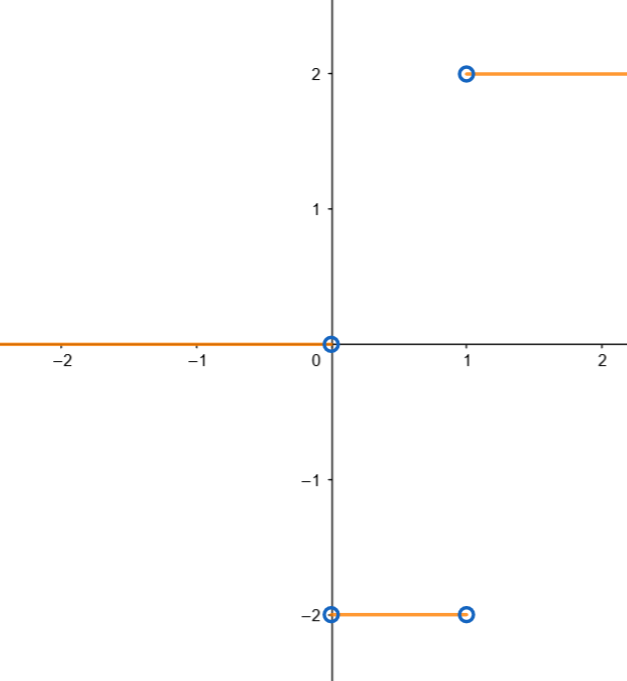
\includegraphics[width=0.8\textwidth]{oef5_heaviside}
\end{center}
}
\section{Exponentiële orde}
Een functie is van exponentiële orde indien $\exists M, a \in R$ zodat $|f(t)| < Me^{at}, \forall t > N$ en met a het minimum van de waarden waarvoor dit geldt. Indien waar is $f(t)$ van exponentiële orde a.
Soms is het gemakkelijker te bewijzen via:
$$\lim_{t \to +\infty} \frac{|f(t)|}{e^{at}} \in R$$
\example{Bepaal de exponentiële orde van $\sin t$}{
\begin{equation*}
\begin{split}
                & |\sin t| \leq 1 \\
\Leftrightarrow & |\sin t| < 1.1 \hbox{(willekeurige waarde)} \\
\Leftrightarrow & |\sin t| < 1.1e^{at}
\end{split}
\end{equation*}
Hieruit kan afgeleid worden dat a = 0 en de exponentiële orde is dus ook 0.
}
\example{Bepaal de exponentiële orde van $(1 + 2t)e^{-t}$}{
Bij deze opgave maken we gebruik van de limietstelling.
\begin{equation*}
\begin{split}
\lim_{t \to +\infty} \frac{|f(t)|}{e^{at}} & = \lim_{t \to +\infty} \frac{|(1 + 2t)e^{-t}|}{e^{at}} \\
                                            & = \lim_{t \to +\infty} \frac{(1 + 2t)e^{-t}}{e^{at}} \\
                                            & = \lim_{t \to +\infty} \frac{1 + 2t}{e^{at}e^{t}} \\
                                            & = \lim_{t \to +\infty} \frac{1 + 2t}{e^{t(a +1)}} 
\end{split}
\end{equation*}
We moeten een onderscheid maak tussen 2 gevallen:
\begin{itemize}
\item $a + 1 < 0 \rightarrow e^{-\infty} = 0 \rightarrow \frac{+\infty}{0} \rightarrow \; \hbox{onbepaald}$
\item $a + 1 > 0 \rightarrow e^{+\infty} = \infty \rightarrow \frac{+\infty}{+\infty} \rightarrow \; \hbox{L'Hopital}$
\end{itemize}
We maken enkel gebruik van het tweede geval en passen dus L'hopital toe.
\begin{equation*}
\begin{split}
\lim_{t \to +\infty} \frac{1 + 2t}{e^{t(a +1)}} & = \lim_{t \to +\infty} \frac{2}{e^{t(a +1)}(a+1)} \\
                                                & = \frac{2}{+\infty} = 0 \in R
\end{split}
\end{equation*}
Aangezien het een reëele uitkomst is kan a uit de uitdrukking $a + 1 > 0$ afgeleid worden.
$$\forall a, a > -1$$
De exponentiële orde is dus -1.
}
\section{De Laplacetransformatie}
Definitie: Stel $f(t)$ causuaal dan is de laplacetransformatie van $f(t)$ een functie die een complex getal $s$ afbeeldt op 
$$\mathcal{L}\{f(t)\}(s) = F(s) = \int_{0}^{+\infty}f(t)e^{-st}\;dt, s \in \mathbb{C}$$
Een voorbeeld uit het formularium:
$$\mathcal{L}\{\sin t\}(s) = \frac{1}{1 + s^2}$$
De letter s kan eender welk complex getal zijn:
$$\mathcal{L}\{\sin t\}(2) = \frac{1}{1 + 4}$$
Indien er een imaginaire eenheid is verandert de definitie minimaal:
$$\mathcal{L}\{\sin t\}(3 + 2j) = \int_{0}^{+\infty}|f(t)e^{-st}|\;dt$$
Het argument tussen de $| ... |$ is NIET de absolute waarde, maar de MODULUS van het complexe getal, te berekenen via $\sqrt{x^2 + y^2}$ indien het complexe getal gedefinieerd wordt als $s = x + yj$ (wat vanaf nu als definitie gebruikt wordt voor een complex getal).
\subsection{Opmerkingen}
\begin{enumerate}
\item $$|f(t)e^{-st}| = |f(t)|e^{-xt}, \; s = x+yj$$
want
\begin{equation*}
\begin{split}
|f(t)e^{-st}| & = |f(t)e^{-(x + yj)t}| \\
                & = |f(t)|\cdot|e^{-(xt + yjt)}| \\
                & = |f(t)|\cdot|e^{-xt} \cdot e^{-yjt}| \\
                & = |f(t)|\cdot|e^{-xt}|\cdot|e^{-yjt}| \\
                & = |f(t)|\cdot e^{-xt}\cdot|\cos(-yt) + j\sin(-yt)| \\
                & = |f(t)|e^{-xt}\sqrt{\cos^2{(-yt)} + \sin^2{(-yt)}} \\
                & = |f(t)|e^{-xt}
\end{split}
\end{equation*}
\item 
$$\mathcal{L}\{af(t) + bg(t)\}(s) = a\mathcal{L}\{f(t)\}(s) + b\mathcal{L}\{g(t)\}(s)$$
De Laplace van een som is gelijk aan de som van een Laplace.
\end{enumerate}
\subsection{Laplacegetransformeerde van enkele basisfuncties}
\begin{itemize}
\item $$\mathcal{L}\{e^{at}\}(s) = \frac{1}{s - a}$$
Bewijs:
\begin{equation*}
\begin{split}
\mathcal{L}\{e^{at}\}(s) & = \int_{0}^{+\infty}e^{at}e^{-st} \; dt \\
                            & = \int_{0}^{+\infty} e^{t(a - s)} \; dt \\
                            & = \frac{e^t{a - s)}}{a - s}\bigg|_{0}^{+\infty} \\
                            & = \frac{1}{a - s}\bigg(\lim_{t \to +\infty}e^{t(a - s)} - 1\bigg)                         
\end{split}
\end{equation*}
Uitwerking van de limiet:
\begin{equation*}
\begin{split}
    \lim_{t \to +\infty}e^{t(a - s)} & = \lim_{t \to +\infty}|e^{at - st)} | \\
                                    & = \lim_{t \to +\infty}|e^{at - (x + yj)t}| \\
                                    & = \lim_{t \to +\infty}|e^{at - xt}\cdot e^{-yjt}| \\
                                    & = \lim_{t \to +\infty}|e^{at - xt}|\cdot |e^{-yjt}| \\
                                    & = \lim_{t \to +\infty}|e^{at - xt}|\cdot |\cos(-yt) + j\sin(-yt)| \\
                                    & = \lim_{t \to +\infty}e^{at - xt}\cdot \sqrt{\cos^2(-yt) + \sin^2(-yt)} \\
                                    & = \lim_{t \to +\infty}e^{at - xt} = e^{-\infty} = 0
\end{split}
\end{equation*}
Deze uitkomst in de oorspronkelijke vergelijking steken:
$$\frac{1}{a - s}(0 - 1) = \frac{1}{s - a}$$ 

\item $$\mathcal{L}\{\sin \omega t\}(s) = \frac{\omega}{\omega^2 + s^2} \qquad  \hbox{en} \qquad  \mathcal{L}\{\cos \omega t\}(s) = \frac{s}{\omega^2 + s^2}$$
Bewijs: We vertrekken van de uitkomst van vorig bewijs. Beschouw $a = wj$
\begin{equation*}
\begin{split}
\mathcal{L}\{e^{wjt}\}(s) & = \frac{1}{s - wj} \\
                            & = \frac{1}{s - wj} \cdot \frac{s + wj}{s + wj} \\
                & = \frac{s + wj}{s^2 + w^2}\\
                & = \mathcal{L}\{\cos (\omega t) + j\sin(\omega t)\}(s) \\
                & = \mathcal{L}\{\cos (\omega t)\}(s) + \mathcal{L}\{j\sin(\omega t) \}(s) \\
                & = \frac{s}{s^2 + w^2} + \frac{w}{s^2 + w^2}j \\ 
\end{split}
\end{equation*}
dus $$\mathcal{L}\{\cos \omega t\}(s) = \frac{s}{\omega^2 + s^2} \qquad  \hbox{en} \qquad  \mathcal{L}\{\sin \omega t\}(s) = \frac{\omega}{\omega^2 + s^2}$$

\item 
$$\mathcal{L}\{\delta(t)\}(s) = 1$$
Bewijs:
\begin{equation*}
\begin{split}
    \mathcal{L}\{\delta(t)\}(s) & = \mathcal{L}\{\delta(t - 0)\}(s) \\
                & = \int_{0}^{+\infty}\delta(t - 0)e^{-st}\;dt \\
                & = f(0) = e^{-s\cdot0} = e^{0} = 1
\end{split}
\end{equation*}
\end{itemize}
\example{Bepaal het laplacebeeld van $\cos{(2t - 1)}$}{
\begin{equation*}
\begin{split}
\mathcal{L}\{\cos(2t - 1)\}(s) & = \mathcal{L}\{\cos(2t)\cos( 1 )+ \sin(2t)\sin (1)\}(s) \\
                & = \cos (1) \mathcal{L}\{\cos 2t\}(s) + \sin (1 )\mathcal{L}\{\sin 2t\}(s)\\
                & = \cos (1) \frac{s}{s^2 + 4} + \sin (1) \frac{2}{s^2 + 4} \\
                & = \frac{s\cos(1)}{s^2 + 4} + \frac{2\sin(1)}{s^2 + 4}
\end{split}
\end{equation*}
}
\example{Bepaal het laplacebeeld van $\sinh(4t) - 3\cos{(\frac{t}{3})}$}
{
\begin{equation*}
\begin{split}
\mathcal{L}\bigg\{\ \sinh(4t) - 3\cos{\bigg(\frac{t}{3}\bigg)} \bigg\}(s) & = \mathcal{L}\bigg\{\ \frac{e^{4t} - e^{-4t}}{2} - 3\cos{\bigg(\frac{t}{3}\bigg)} \bigg\}(s) \\
& = \mathcal{L}\bigg\{\ \frac{e^{4t} - e^{-4t}}{2}\bigg\}(s) - 3\mathcal{L}\bigg\{\cos{\bigg(\frac{t}{3}\bigg)} \bigg\}(s) \\
& = \frac{1}{2}\bigg(\frac{1}{s - 4} - \frac{1}{s + 4}\bigg) - 3\frac{s}{s^2 + \frac{1}{9}} \\
& = \frac{1}{2}\bigg(\frac{1}{s - 4} - \frac{1}{s + 4}\bigg) - \frac{27s}{9s^2 + 1}
\end{split}
\end{equation*}
}
\example{Bepaal het laplacebeeld van $\delta(t - \frac{\pi}{2})\cos(4t)e^{2t}$}{
\begin{equation*}
\begin{split}
\mathcal{L}\bigg\{\delta\bigg(t - \frac{\pi}{2}\bigg)\cos(4t)e^{2t}\bigg\}(s) & = \int_{0}^{+\infty}\cos(4t)e^{2t}\delta\bigg(t - \frac{\pi}{2}\bigg)e^{-st} \; dt \\
& = f\bigg(\frac{\pi}{2}\bigg) \\
& = \cos\bigg(4 \cdot \frac{\pi}{2}\bigg)e^{2\cdot\frac{\pi}{2}}e^{-s\cdot\frac{\pi}{2}} \\
& = \cos(2\pi)e^{\pi}e^{-\frac{s\pi}{2}}\\
& = e^{\pi}e^{-\frac{s\pi}{2}}
\end{split}
\end{equation*}

}
\subsection{Translatie naar rechts}
Definitie:
$$\mathcal{L}\{f(t - a)H(t - a)\}(s) = e^{-as}F(s) \qquad a > 0$$
Bewijs:
\begin{equation*}
\begin{split}
\mathcal{L}\{f(t - a)H(t - a)\}(s) & = \int_{0}^{+\infty}f(t - a)H(t - a)e^{-st} \; dt \\
                                    & = \int_{0}^{a}f(t - a)H(t - a)e^{-st} \; dt + \int_{a}^{+\infty}f(t - a)H(t - a)e^{-st} \; dt \\
                                    & = 0 +\int_{a}^{+\infty}f(t - a)H(t - a)e^{-st} \; dt \\
                                    & = \int_{a}^{+\infty}f(t - a)H(t - a)e^{-st} \; dt \\
                                    \hbox{stel}\quad u & = t - a \\
                                    \hbox{dan}\quad du & = dt \\    
                                    & = \int_{0}^{+\infty}f(u)e^{-s(u + a)} \; du \\
                                    & = \int_{0}^{+\infty}f(u)e^{-su}e^{-sa} \; du \\
                                    & = e^{-sa}\int_{0}^{+\infty}f(u)e^{-su} \; du \\
                                    & = e^{-sa}\mathcal{L}\{f(t)\}(s) \\
                                    & = e^{-as}F(s)
\end{split}
\end{equation*}
\example{Bepaal het laplacebeeld van $f(t) = (t^2 - 1)H(t - 1) - \sin(3t)H(t - \pi)$}
{
\begin{equation*}
\begin{split}
\mathcal{L}\{f(t)\} & = \mathcal{L}\{(t^2 - 1)H(t - 1)\}(s) - \mathcal{L}\{\sin(3t)H(t-\pi)\}(s)
\end{split}
\end{equation*}
We werken beide laplacetransformaties afzonderlijk uit:
\begin{equation*}
\begin{split}
%t^2 - 1 = (t - 1)^2 + 2t - 2 = (t - 1)^2 + 2(t - 1)%
\mathcal{L}\{(t^2 - 1)H(t - 1)\}(s) & = \mathcal{L}\{[(t-1)^2 + 2(t - 1)]H(t - 1)\}(s)\\
                                    & = e^{-as}\mathcal{L}\{t^2 + 2t\}(s) \\
                                    & = e^{-s}\bigg(\frac{2!}{s^3} + 2\frac{1!}{s^2}\bigg) \\
                                    & = e^{-s}\bigg(\frac{2}{s^3} + \frac{2}{s^2}\bigg)\\
                                    & = e^{-s}\bigg(\frac{2(1 + s)}{s^3}\bigg)
\end{split}
\end{equation*}
\begin{equation*}
\begin{split}
    %sin 3t = sin(3(t - \pi)) + 3\pi) = sin(3(t - \pi) + \pi) = -sin(3(t-\pi))%
\mathcal{L}\{\sin(3t)H(t-\pi)\}(s) & =  \mathcal{L}\{-\sin(3(t - \pi))H(t-\pi)\}(s) \\
                                    & = -e^{-\pi s}\mathcal{L}\{\sin (3t)\}(s) \\
                                    & = -e^{-\pi s}\frac{3}{s^2 + 9} \\
                                    & = -\frac{3e^{-\pi s}}{s^2 + 9}
\end{split}
\end{equation*}
Het resultaat wordt:
\begin{equation*}
\begin{split}
\mathcal{L}\{f(t)\} & = \mathcal{L}\{(t^2 - 1)H(t - 1)\}(s) - \mathcal{L}\{\sin(3t)H(t-\pi)\}(s) \\
                    & = e^{-s}\bigg(\frac{2(1 + s)}{s^3}\bigg) - \bigg(-\frac{3e^{-\pi s}}{s^2 + 9}\bigg) \\
                    & = e^{-s}\bigg(\frac{2(1 + s)}{s^3}\bigg) +\frac{3e^{-\pi s}}{s^2 + 9}
\end{split}
\end{equation*}
}
\subsection{Dempingsfunctie}
Definitie:
$$\mathcal{L}\{e^{-at}f(t)\}(s) = F(s + a)$$
\example{Bepaal het laplacebeeld van $f(t) = t(t^3 - 1)^2e^{-t} + \sin(\sqrt{3}t)e^{2t}$}
{
\begin{equation*}
\begin{split}
\mathcal{L}\{f(t)\}(s) = \mathcal{L}\{t(t^3 - 1)^2e^{-t}\}(s) + \mathcal{L}\{\sin(\sqrt{3}t)e^{2t}\}(s)
\end{split}
\end{equation*}
Ook hier beschouwen we beide laplacetransformaties apart.
\begin{equation*}
\begin{split}
\mathcal{L}\{t(t^3 - 1)^2e^{-t}\}(s) & = \mathcal{L}\{(t^7 - 2t^4 + t)e^{-t}\}(s) \\
                                    & = \mathcal{L}\{t^7 - 2t^4 + t\}(s + 1) \\
                                    & = \frac{7!}{(s + 1)^8} - \frac{2 \cdot 4!}{(s + 1)^5} + \frac{1!}{(s + 1)^2} \\
                                    & = \frac{7!}{(s + 1)^8} - \frac{48}{(s + 1)^5} + \frac{1}{s^2 + 2s + 1}
\end{split}
\end{equation*}
\begin{equation*}
\begin{split}
\mathcal{L}\{\sin(\sqrt{3}t)e^{2t}\}(s) & = \mathcal{L}\{\sin(\sqrt{3}t)\}(s - 2) \\
                                        & = \frac{\sqrt{3}}{(s - 2)^2 + 3} \\
                                        & = \frac{\sqrt{3}}{s^2 -2s + 7}
\end{split}
\end{equation*}
Het resultaat wordt:
\begin{equation*}
\begin{split}
\mathcal{L}\{f(t)\}(s) & = \mathcal{L}\{t(t^3 - 1)^2e^{-t}\}(s) + \mathcal{L}\{\sin(\sqrt{3}t)e^{2t}\}(s) \\
                        & = \frac{7!}{(s + 1)^8} - \frac{48}{(s + 1)^5} + \frac{1}{s^2 + 2s + 1} + \frac{\sqrt{3}}{s^2 -2s + 7}
\end{split}
\end{equation*}
}
\subsection{Schaalwijziging}
Definitie:
$$\mathcal{L}\{f(at)\}(s) = \frac{1}{a}F(\frac{s}{a})$$
Bewijs:
\begin{equation*}
 \begin{split}
  \mathcal{L}\{f(at)\}(s) & = \int_{0}^{+\infty}f(at)e^{-st}\;dt \\
                    \hbox{stel}\; u & = at \\
                    \hbox{dan}\; du & = adt \\
                          & =  \int_{0}^{+\infty}f(u)e^{-s\frac{u}{a}}\;\frac{du}{a} \\
                          & =  \frac{1}{a}\int_{0}^{+\infty}f(u)e^{-\frac{s}{a}u}\;du \\
                          & =  \frac{1}{a}\mathcal{L}\{f(u)\}(\frac{s}{a}) \\
                          & =  \frac{1}{a}F(\frac{s}{a})
 \end{split}
\end{equation*}
\example{Gegeven $\mathcal{L}\{\sin t\}(s) = \frac{1}{s^2 + 1}$. Bepaal $\mathcal{L}\{\sin \omega t\}(s)$}
{
\begin{equation*}
 \begin{split}
  \mathcal{L}\{f(\omega t)\}(s) & = \mathcal{L}\{\sin \omega t\}(s) \\
                                & = \frac{1}{\omega}\mathcal{L}\{\sin t\}(\frac{s}{\omega}) \\
                                & = \frac{1}{\omega}\frac{1}{\frac{s^2}{\omega^2} + 1} \\
                                & = \frac{\omega}{\omega^2(\frac{s^2}{w^2} + 1)} \\
                                & = \frac{\omega}{s^2 + w^2}
 \end{split}
\end{equation*}}
\subsection{Laplacegetransformeerde van f'(t)}
Definitie:
$$\mathcal{L}\bigg\{\frac{df(t)}{dt}\bigg\}(s) = sF(s) - f(0^+), \forall s \in \mathbb{C}, Re(s) > a$$
\example{Gegeven $\mathcal{L}\{\sin \omega t\}(s) = \frac{\omega}{s^2 + w^2}$. Bepaal $\mathcal{L}\{\cos\omega t\}(s)$. }{
\begin{equation*}
 \begin{split}
  \mathcal{L}\{\cos\omega t\}(s) & = \mathcal{L}\bigg\{\frac{d[\sin \omega t]}{dt}\bigg\}(s) \\
                                 & = s\mathcal{L}\{\sin \omega t\}(s) - \sin{\omega \cdot 0} \\
                                 & = s\frac{\omega}{s^2 + w^2}
 \end{split}
\end{equation*}
\begin{equation*}
 \begin{split}
                  & \mathcal{L}\{\omega \cos\omega t\}(s) = s\frac{\omega}{s^2 + w^2} \\
  \Leftrightarrow & \omega \mathcal{L}\{\cos\omega t\}(s) = \omega\frac{s}{s^2 + w^2} \\
  \Leftrightarrow & \mathcal{L}\{\cos\omega t\}(s) = \frac{s}{s^2 + w^2} \\
 \end{split}
\end{equation*}}
\subsection{Laplacegetransformeerde van f''(t)}
Definitie:
$$\mathcal{L}\{f^{(n)}(t)\}(s) = s^nF(s) - s^{n - 1}f(0^+) - s^{n -2}f'(0^+) - ... - sf^{(n - 2)}(0^+) - f^{(n-1)}(0^+)$$
\example{Gegeven $g(t) = te^{-t}$, bepaal $\mathcal{L}\{g''(t)\}(s)$}{
\begin{equation*}
 \begin{split}
  \mathcal{L}\{g''(t)\}(s) & = \mathcal{L}\bigg\{\frac{d^2g}{dt^2}\bigg\}(s) \\
                           & = s^2G(s) - sg(0^+) - g'(t) \\
                           \hbox{met}\;G(s) & = \mathcal{L}\{te^{-t}\}(s) \\
                                            & = \mathcal{L}\{t\}(s + 1) \\
                                            & = \frac{1}{(s+1)^2}  \\
                           \hbox{en}\; g'(t)  & = -te^{-t} + e^{-t} \\
                                                     & = e^{-t}(1 - t) \\
            \Rightarrow s^2G(s) - sg(0^+) -  g'(0)  & = s^2\frac{1}{(s+1)^2} - s\cdot0 - 1 \\
            & = \frac{-2s - 1}{(s + 1)^2}
 \end{split}
\end{equation*}
}
\subsection{Laplacegetransformeerde van machten van t}
Definitie:
$$\mathcal{L}\{t^nf(t)\}(s) = (-1)^n\frac{d^nF(s)}{ds^n}$$
Bewijs:
\begin{equation*}
 \begin{split}
  F(s) & = \int_0^{+\infty}f(t)e^{-st}\; dt \\
  \frac{dF}{ds} & = \int_0^{+\infty}-tf(t)e^{-st}\; dt  \\
                & = -\int_0^{+\infty}tf(t)e^{-st}\; dt  \\
                & = -\mathcal{L}\{tf(t)\}(s)  \\
  \frac{d^2F}{ds^2} & = -\int_0^{+\infty}(-t)tf(t)e^{-st}\; dt  \\
                    & = \int_0^{+\infty}t^2f(t)e^{-st}\; dt  \\
                    & = \mathcal{L}\{t^2f(t)\}(s)  \\
 \end{split}
\end{equation*}
\example{Bepaal $\mathcal{L}\{t \sin t - t^3e^{-t}\}(s)$}{
\begin{equation*}
 \begin{split}
  \mathcal{L}\{t \sin t - t^3e^{-t}\}(s) & = \mathcal{L}\{t \sin t\}(s) - \mathcal{L}\{t^3e^{-t}\}(s)\\
  *) \mathcal{L}\{t \sin t\}(s) & = (-1)^1\frac{d\mathcal{L}\{\sin t\}(s)}{ds} \\
                                & =  -\frac{d\big(\frac{1}{1 + s^2}\big)}{ds} \\
                                & = -\bigg(\frac{-2s}{(1+s^2)^2}\bigg) \\
                                & = \frac{2s}{(1+s^2)^2} \\
**) \mathcal{L}\{t^3e^{-t}\}(s) & = (-1)^3\frac{d^3\mathcal{L}\{e^{-t}\}(s)}{ds^3} \\
                                & = -\frac{d^3\mathcal{L}\{e^{-t}\}}{ds^3} \\
                                & = -\frac{d^3\big(\frac{1}{s + 1}\big)}{ds^3} \\
                                & = -\frac{d^3[(s + 1)^{-1}]}{ds^3} \\
                            \frac{dF}{ds} & = -(s+1)^{-2} \\
                            \frac{d^2F}{ds^2} & = 2(s+1)^{-3} \\
                            \frac{d^3F}{ds^3} & = -6(s+1)^{-4} \\
                            \Rightarrow -\frac{d^3[(s + 1)^{-1}]}{ds^3} & = -(-6(s+1)^{-4} \\
                            & = \frac{6}{(s+1)^4}\\
 * - ** & = \frac{2s}{(1+s^2)^2} - \frac{6}{(s+1)^4}
 \end{split}
\end{equation*}}
\subsection{Laplacegetransformeerde van een integraal}
Definitie:
$$\mathcal{L}\bigg\{\int_0^tf(u)\;du\bigg\}(s) = \frac{1}{s}F(s) \forall s \in \mathbb{C}, Re(s) > a$$
Bewijs:
\begin{equation*}
 \begin{split}
  g(t) & = \int_{0}^{t}f(u)\;du \\
  g't) & = f(t) \\
  g'(0) & = 0 \\
  \Rightarrow \mathcal{L}\{g'(t)\}(s) & = sG(s) - g(0^+) \\
  \Rightarrow \mathcal{L}\{f(t)\}(s) & = s\mathcal{L}\bigg\{\int_0^tf(u)\;du\bigg\}(s) - 0 \\
  \Rightarrow \frac{1}{s}F(s) & = \mathcal{L}\bigg\{\int_0^tf(u)\;du\bigg\}(s)
 \end{split}
\end{equation*}
\example{Bepaal $\mathcal{L}\bigg\{\int_0^t  \cos \omega t \; dt\bigg\}$}{
\begin{equation*}
 \begin{split}
  \mathcal{L}\bigg\{\int_0^t  \cos \omega t \; dt\bigg\} & = \frac{1}{s}\mathcal{L}\{\sin \omega t\}(s) \\
                                                         & = \frac{1}{s}\frac{s}{s^2 + \omega^2} \\
                                                         & = \frac{1}{s^2 + \omega^2}
 \end{split}
\end{equation*}
}
\subsection{Laplacegetransformeerde van een periodische functie}
Definitie:
$$\mathcal{L}\{f(t)\}(s) = \frac{1}{1 - e^{-sT}}\int_0^{T}e^{-st}f(t)\; dt$$
\todo{slide 19}
\subsection{De convolutiestelling}
Definitie:
$$(f * g)(t) = \int_0^t f(u)g(t - u)\;du$$
Hieruit volgt:
$$
\mathcal{L}\{(f * g)(t)\}(s) = F(s)G(s)$$
Bewijs(niet te kennen)

\example{Gegeven $f(t) = e^{at}$ en $g(t) = e^{bt}$. Illustreer de juistheid van deze rekenregel.}{
\begin{equation*}
 \begin{split}
    f(t) * g(t) & = e^{at} e^{bt} \\
                & = \int_{0}^{t} e^{au}e^{b(t-u}\; du\\
                & = \int_{0}^{t} e^{au}e^{bt}e^{-bu}\; du\\
                & = e^{bt}\int_{0}^{t} e^{au}e^{-bu}\; du\\
                & = e^{bt}\int_{0}^{t} e^{u(a-b)}\; du\\
                & = e^{bt}\bigg[\frac{e^{u(a-b)}}{a - b}\bigg]_0^t\\
                & = \frac{e^{bt}}{a - b}[e^{t(a-b)} - 1] \\
                & = \frac{1}{a - b}(e^{at} - e^{bt}) \\
    \Rightarrow \mathcal{L}\{\frac{1}{a - b}(e^{at} - e^{bt})\}(s) & = \frac{1}{a - b}\mathcal{L}\{(e^{at} - e^{bt})\}(s) \\
                                                                   & = \frac{1}{a - b}\bigg(\frac{1}{s-a} - \frac{1}{s - b}\bigg) \\
                                                                   & = \frac{1}{a - b}\bigg(\frac{(s - b) - (s - a)}{(s - a)(s - b)}\bigg) \\
                                                                   & = \frac{1}{s - a}\frac{1}{s - b} \\
                                                                   & = \mathcal{L}\{e^{at}\}(s)\mathcal{L}\{e^{bt}\}(s)
 \end{split}
\end{equation*}
}
\example{Bereken $H(t)*H(t)*H(t)$.}{
\begin{equation*}
 \begin{split}
  H(t) * H(t) & = (H * H)(t) \\
              & = \int_0^t H(u)H(t - u)\; du \\
            \hbox{aangezien}\; & 0 \leq u \leq t \\
            \Rightarrow & H(u)  = 1 \\
            \Rightarrow & H(t - u)  = 1 \\
              & = \int_0^t \; du \\
              & = [u]_0^t \\
              & = t
 \end{split}
\end{equation*}
\begin{equation*}
 \begin{split}
  H(t) * H(t) * H(t) & = (H * H)(t) * H(t) \\
                     & = t * H(t) \\
                     & = \int_0^t uH(t - u)\; du \\
                     & = \bigg[\frac{u^2}{2}\bigg]_0^t \\
                     & = \frac{t^2}{2}       
 \end{split}
\end{equation*}


}
\subsection{Inverse Laplacetransformatie}
Definitie:
$$\mathcal{L}^{-1}\{F(s)\}(t) = f(t) \qquad \hbox{indien} \qquad \mathcal{L}\{f(t)\}(s) = F(s)$$
\example{Bepaal het invers laplacebeeld van 
        $$\frac{s^2 + 2s + 1}{s(s-1)(s-2)}$$
    }{
        \begin{equation*}
         \begin{split}
          \mathcal{L}^{-1}\{\frac{s^2 + 2s + 1}{s(s-1)(s-2)}\}(t) & = \mathcal{L}^{-1}\{\frac{a}{s} + \frac{b}{s-1} + \frac{c}{s-2}\}(t) \\
                                                                  & = \mathcal{L}^{-1}\{\frac{a(s-1)(s-2) + bs(s-2) + cs(s-1)}{s(s-1)(s-2)}\}(t) \\
                                                       \Rightarrow s^2 + 2s + 1 & = a(s-1)(s-2) + bs(s-2) + cs(s-1) \\
                                                            \hbox{als}\;s = 0 & : a = \frac{1}{2} \\
                                                            \hbox{als}\;s = 1 & : b = -4\\
                                                            \hbox{als}\;s = 2 & : c = \frac{9}{2} \\     
                                                                  & = \mathcal{L}^{-1}\{\frac{1/2}{s} + \frac{-4}{s-1} + \frac{9/2}{s-2}\}(t) \\
                                                                  & = \frac{1}{2} + (-4e^{t}) + \frac{9}{2}e^{2t} \\
                                                                  & = \frac{1}{2}(1 - 8e^{t} + 9e^{2t})
         \end{split}
        \end{equation*}
    }
\example{Bepaal het invers laplacebeeld van
    $$\frac{s^2 - 2}{2s^2 + 4s + 10}$$
}{
    \begin{equation*}
     \begin{split}
      \mathcal{L}^{-1}\{\frac{s^2 - 2}{2s^2 + 4s + 10}\} & = \mathcal{L}^{-1}\bigg\{\frac{1}{2} - \frac{2s + 7}{2s^2 + 4s + 10}\bigg\}   \\
                                                    & = \mathcal{L}^{-1}\bigg\{\frac{1}{2} - \frac{s + 7/2}{s^2 + 2s + 5}\bigg\}    \\
                                                    & = \mathcal{L}^{-1}\bigg\{\frac{1}{2} - \frac{s + 7/2}{(s+1)^2 + 4}\bigg\}  \\
                                                    & = \mathcal{L}^{-1}\bigg\{\frac{1}{2} - \frac{(s + 1) + 5/2}{(s+1)^2 + 4}\bigg\}  \\
                                                    & = \mathcal{L}^{-1}\bigg\{\frac{1}{2} - \frac{s + 1}{(s+1)^2 + 4} - \frac{5}{2}\frac{1}{(s+1)^2 + 4}\bigg\}  \\
                                                    & = \mathcal{L}^{-1}\bigg\{\frac{1}{2}\bigg\} - \mathcal{L}^{-1}\bigg\{\frac{s + 1}{(s+1)^2 + 4}\bigg\} - \frac{5}{2}\mathcal{L}^{-1}\bigg\{\frac{1}{(s+1)^2 + 4}\bigg\}  \\
                                                    & = \frac{1}{2}\delta(t) - \cos(2t)e^{-t} - \frac{5}{2}\sin(2t)e^{-t} \\
                                                    & = \frac{1}{2}\delta(t) - e^{-t}(\cos 2t + \frac{5}{2}\sin 2t)
     \end{split}
    \end{equation*}

}
\example{Bepaal het invers laplacebeeld van 
    $$\frac{e^{-\pi s}}{(s+1)(s^2+2s+2)}$$
}{
    \begin{equation*}
     \begin{split}
      \mathcal{L}^{-1}\bigg\{\frac{e^{-\pi s}}{(s+1)(s^2+2s+2)}\bigg\}(t)
                                                                       & = \mathcal{L}^{-1}\bigg\{\frac{1}{(s+1)(s^2+2s+2)}\cdot e^{-\pi s}\bigg\}(t) \\
                                                                       & = f(t - \pi)H(t - \pi)  \\
                                                                       \hbox{met}\; f(t) & = \mathcal{L}^{-1}\bigg\{\frac{1}{(s+1)(s^2+2s+2)}\bigg\}(t) \\
                                                                       \Rightarrow \frac{1}{(s+1)(s^2+2s+2)} & = \frac{a}{s + 1} + \frac{b + cs}{s^2 + 2s + 2} \\
                                                                                                             & = \frac{a(s^2 + 2s + 2) + (b+cs)(s+1)}{(s+1)(s^2+2s+2)}   \\
                                                                       \Rightarrow 1 & = a(s^2 + 2s + 2) + (b+cs)(s+1) \\
                                                                       \begin{cases}
                                                                        2a + b = 1  \\
                                                                        2a + b + c = 0 \\ 
                                                                        a + c = 0 \\
                                                                       \end{cases} 
                                                                       & \Rightarrow
                                                                       \begin{cases}
                                                                        a = 1  \\
                                                                        b = -1\\ 
                                                                        c = -1 \\
                                                                       \end{cases} \\
                                                                       \Rightarrow \mathcal{L}^{-1}\bigg\{\frac{1}{(s+1)(s^2+2s+2)}\bigg\}(t) & = \mathcal{L}^{-1}\bigg\{\frac{1}{s + 1} + \frac{s + 1}{s^2 + 2s + 2}\bigg\}(t) \\                  
                                                                       & = \mathcal{L}^{-1}\bigg\{\frac{1}{s + 1} + \frac{s + 1}{(s+1)^2 + 1}\bigg\}(t) \\    
                                                                       & = e^{-t} - \cos(t) e^{-t} \\
                                                                       & = e^{-t}( 1 - \cos t) = f(t) \\
                                                                       \hbox{ANTWOORD}\Rightarrow & e^{-(t - \pi)}(1 - \cos(t - \pi)H(t - \pi) \\
                                                                                 = & e^{\pi - t}(1 + \cos t)H(t - \pi)
     \end{split}
    \end{equation*}

}
\example{Bepaal het inverse laplacebeeld van 
    $$\frac{e^{2s}}{(s-3)^6}$$
}{
    \begin{equation*}
     \begin{split}
      \mathcal{L}^{-1}\bigg\{\frac{e^{2s}}{(s-3)^6}\bigg\}(t) & = f(t-2)H(t - 2) \\ 
                                                    \hbox{met} \; f(t) & = \mathcal{L}^{-1}\bigg\{\frac{1}{(s-3)^6}\bigg\}(t) \\
                                                                       & = g(t)e^{3t} \\
                                                    \hbox{met} \; g(t) & = \mathcal{L}^{-1}\bigg\{\frac{1}{s^6}\bigg\}(t) \\
                                                                       & = \frac{1}{5!}\mathcal{L}^{-1}\bigg\{\frac{5!}{s^6}\bigg\}(t) \\
                                                                       & = \frac{t^5}{5!} \\
                                                    f(t) & = g(t)e^{3t} \\
                                                         & = \frac{t^5e^{3t}}{5!} \\
     \mathcal{L}^{-1}\bigg\{\frac{e^{2s}}{(s-3)^6}\bigg\}(t) & = f(t-2)H(t - 2) \\ 
                                                             & = \frac{(t-2)^5e^{3(t-2)}}{5!}H(t-2)
     \end{split}
    \end{equation*}

}
\example{Bereken $(H*H*H*H*)(t)$}
{
    \begin{equation*}
     \begin{split}
      (H*H*H*H*)(t) & = \frac{1}{s^4} \\
                    & = \frac{1}{3!}\mathcal{L}^{-1}\bigg\{\frac{3!}{s^4}\bigg\}(t) \\
                    & = \frac{t^3}{6}
     \end{split}
    \end{equation*}

}
\example{Bereken:
    $$\mathcal{L}^{-1}\bigg\{\frac{s}{(s^2 + 4)^2}\bigg\}(t)$$
}{
    \begin{equation*}
     \begin{split}
      \mathcal{L}^{-1}\bigg\{\frac{s}{(s^2 + 4)^2}\bigg\}(t) & = \mathcal{L}^{-1}\bigg\{\frac{s}{(s^2 + 4)}\frac{1}{(s^2 + 4)}\bigg\}(t) \\
                                                             & = \frac{1}{2}\mathcal{L}^{-1}\bigg\{\frac{s}{(s^2 + 4)}\frac{2}{(s^2 + 4)}\bigg\}(t) \\
                                                             & = \frac{1}{2}(\sin 2t * \cos 2t) \\
                                                             & = \frac{1}{2}\int_0^t \sin 2u \cos [2(t - u)] \; du\\
                                                             & = \frac{1}{4}\int_0^t \sin(2u - [2(t - u)]) + \sin(2u + [2(t - u)])\; du \\
                                                             & = \frac{1}{4} \int_0^t \sin(4u - 2t) + \sin 2t\; du \\
                                                             & = \frac{1}{4}\bigg[ \int_0^t \sin(4u - 2t) \; du  + \int_0^t \sin 2t\; du \bigg] \\
                                                             & = \frac{1}{16}\bigg[-\cos(4u - 2t)\bigg]_0^t + \frac{1}{4}\bigg[u\sin 2t\bigg]_0^t \\
                                                             & = \frac{1}{16}\bigg(-\cos 2t + \cos (-2t)\bigg) + \frac{1}{4}t\sin 2t \\
                                                             & =\frac{1}{4}t\sin 2t
     \end{split}
    \end{equation*}

}










\chapter{Reeksen}
\section{Definities}
Rij [$a_n$] = $a_1, a_2, ..., a_n, ...$ met $a_n$ de algemene term.

$$
	[a_n] =
	\begin{cases}
		\hbox{convergent als }  \lim\limits_{n\to\infty} a_n \in \mathbb{R}              \\
		\hbox{divergent naar } \infty \hbox{ als } \lim\limits_{n\to\infty} a_n = \infty \\
		\hbox{divergent als } \lim\limits_{n\to\infty} a_n = ?
	\end{cases}
$$

\example{
	$$\big[\ln(\frac{1}{n})\big]$$
}{
	$$\lim\limits_{n\to\infty} \ln(\frac{1}{n}) = \ln(0^+) = -\infty$$
	Dus divergent naar $-\infty$.
}
\example{
	$$\big[(1 - \frac{1}{n})^n\big]$$
}{
	$$\lim\limits_{n\to\infty} (1 - \frac{1}{n})^n = 1^\infty$$
	Dit is een onbepaaldheid. We maken gebruik van het getal $e$.
	$$=\lim\limits_{n\to\infty} \bigg(1 + \big(-\frac{1}{n}\big)\bigg)^{n(-1)} = e^{-1}$$
	Dus convergent.
}
\example{
	$$2, -1, \frac{1}{2}, -\frac{1}{4}, ..., ...$$
}{
	Bepaal de algemene term: $a_n = 2\bigg(-\frac{1}{2}\bigg)^{n - 1}$
	$$\lim\limits_{n\to\infty} 2\bigg(-\frac{1}{2}\bigg)^{n - 1} = 2\cdot0 = 0$$
	Dus convergent.
}
\example{
	$$[(-2)^n]$$
}{
	$$[(-2)^n] = -2, 4, -8, 16, -32, ...$$
	De laatste term is ofwel positief ofwel negatief. De limiet bestaat niet dus deze reeks is divergent.
}

\section{Hoofdeigenschappen}
Een stijgende rij naar boven begrensd is convergent. Een dalende rij naar onder begrensd is convergent.

In symbolen:

$$a_n \uparrow, \forall n \quad a_n \leq b \rightarrow \hbox{ convergent}$$
$$a_n \downarrow, \forall n \quad b \leq a_n  \rightarrow \hbox{ convergent}$$

\example{
	$$\bigg[\frac{2n - 1}{n}\bigg]$$
}{
	Als $n$ stijgt zal $\frac{1}{n}$ dalen. $2 - \frac{1}{n}$ stijgt dus.
	Er kan besloten worden dat voor alle $n$ dat $2 - \frac{1}{2} \leq 2$. Deze reeks convergeert
}
\example{
	$$\bigg[\sin\frac{1}{n}\bigg]$$
}{
	Als $n$ stijgt zal $\frac{1}{n}$ dalen. $\sin\frac{1}{n}$ daalt dus.
	Er kan besloten worden dat voor alle $n$ dat $\sin\frac{1}{n} \geq 0$. Deze reeks convergeert.
}

\section{Numerieke reeksen}
$$\sum_{n=0}^{\infty} a_n = a_1 + a_2 + a_3 + ... + a_n$$
waarbij
\begin{itemize}
	\item $S_1 = a_1$
	\item $S_2 = a_1 + a_2$
	\item $S_3 = a_1 + a_2 + a_3$
	\item $S_n = a_1 + a_2 + a_3 + ... + a_n$
\end{itemize}
$$
	\sum a_n =
	\begin{cases}
		\hbox{convergent als }  \lim\limits_{n\to\infty} S_n \in \mathbb{R}              \\
		\hbox{divergent naar } \infty \hbox{ als } \lim\limits_{n\to\infty} S_n = \infty \\
		\hbox{divergent als } \lim\limits_{n\to\infty} S_n = ?
	\end{cases}
$$
\example{
	Bewijs dat de volgende reeks convergent of divergent is:
	$$\sum_{n = 2}^{\infty}\bigg(\frac{1}{\sqrt{n - 1}} - \frac{1}{\sqrt{n + 1}}\bigg)$$
}{
	Uitschrijven van een aantal partieelsommen:
	\begin{itemize}
		\item n = 2: $S_1 = \frac{1}{\sqrt{1}} - \frac{1}{\sqrt{3}} = 1 - \frac{1}{\sqrt{3}}$
		\item n = 3: $S_2 = 1 - \frac{1}{\sqrt{3}} + \frac{1}{\sqrt{2}} - \frac{1}{\sqrt{4}}$
		\item n = 4: $S_3 = 1 - \frac{1}{\sqrt{3}} + \frac{1}{\sqrt{2}} - \frac{1}{\sqrt{4}} + \frac{1}{\sqrt{3}} - \frac{1}{\sqrt{5}} = 1 + \frac{1}{\sqrt{2}} - \frac{1}{\sqrt{4}} - \frac{1}{\sqrt{5}}$
		\item n = 5: $S_4 = 1 + \frac{1}{\sqrt{2}} - \frac{1}{\sqrt{4}} - \frac{1}{\sqrt{5}} + \frac{1}{\sqrt{4}} - \frac{1}{\sqrt{6}} = 1 + \frac{1}{\sqrt{2}} - \frac{1}{\sqrt{5}} - \frac{1}{\sqrt{6}}$
	\end{itemize}
	Hieruit volgt dat
	$$S_n = 1 + \frac{1}{\sqrt{2}} - \frac{1}{\sqrt{n + 1}} - \frac{1}{\sqrt{n + 2}}$$
	Berekening van de limiet:
	$$\lim\limits_{n\to\infty}S_n = 1 + \frac{1}{\sqrt{2}} - 0 - 0 = 1 + \frac{1}{\sqrt{2}}$$
	De reeks convergeert.
}
\example{
	Bewijs dat de volgende reeks convergent of divergent is:
	$$\sum_{n = 0}^{\infty}(-1)^n$$
}{
	Uitschrijven van een aantal partieelsommen:
	\begin{itemize}
		\item n = 0: $S_1 = 1$
		\item n = 1: $S_2 = 1 - 1 = 0$
		\item n = 2: $S_3 = 0 + 1 = 1$
		\item n = 3: $S_4 = 1 - 1 = 0$
	\end{itemize}
	Hieruit volgt dat
	$$S_{2n} = 0 \qquad \hbox{en} \qquad S_{2n + 1} = 1$$
	De limiet bestaat niet dus de reeks divergeert.
}

\section{De meetkundige reeks}
$$\sum_{n = 0}^{\infty} q^n = 1 + q + q^2 + ... + q^{n - 1} + ...$$
\subsection{Convergentieonderzoek}
We weten dat
$$S_n = 1 + q + ... + q^{n - 1} = \frac{1 - q^n}{1 - q}$$
We moeten de limiet van $S_n$ berekenen. We onderscheiden twee gevallen:
\begin{itemize}
	\item $q \neq 1$
	      $$\lim\limits_{n\to\infty}\frac{1 - q^n}{1 - q} = \frac{1}{1 - q}(1 - \lim\limits_{n\to\infty} q^n)$$
	      \begin{itemize}[label={als}]
		      \item $|q| < 1 \Rightarrow \lim\limits_{n\to\infty} q^n = 0$
		            dus
		            $\lim\limits_{n\to\infty} S_n = \frac{1}{1 - q}(1 - 0) = \frac{1}{1 - q} \in \mathbb{R}$

		            Convergent
		      \item $|q| > 1 \Rightarrow \lim\limits_{n\to\infty} q^n = +\infty$
		            dus
		            $\lim\limits_{n\to\infty} S_n = +\infty$

		            Divergent naar $+\infty$
		      \item $q \leq 1 \Rightarrow \lim\limits_{n\to\infty} q^n = ?$

		            Divergent
	      \end{itemize}
	\item $q = 1$
	      $$\sum_{n = 0}^{\infty} 1^n = \sum_{n = 0}^{\infty} 1$$
	      $$S_n = n \rightarrow \lim\limits_{n\to\infty} S_n = \lim\limits_{n\to\infty} n = +\infty$$

	      Divergent naar $+\infty$
\end{itemize}

Uit dit onderzoek volgt het volgende:
$$
	\boxed{
		\sum_{n = 0}^{\infty} q^n = \begin{cases}
			|q| < 1 \rightarrow \hbox{Convergent}               \\
			q \geq 1 \rightarrow \hbox{Divergent naar } +\infty \\
			q \leq -1 \rightarrow \hbox{Divergent}
		\end{cases}
	}
$$

\example{
	Convergeert de reeks $-2 + \frac{2}{3} - \frac{2}{9} + \frac{2}{27} - \frac{2}{81} + ...$ en indien convergent, naar welke reekssom?
}{
	Herschrijf de reeks:
	$$-2(1 - \frac{1}{3} + \frac{1}{9} - \frac{1}{27} + \frac{1}{81} - ... + \bigg(\frac{1}{3}\bigg)^n + ...$$
	Dit komt overeen met
	$$-2\sum_{n = 0}^{\infty}\bigg(-\frac{1}{3}\bigg)^n$$
	Dit is een meetkundige reeks met $q = -\frac{1}{3}$. Het is duidelijk dat $|q| < 1$ dus de reeks convergeert. De reekssom is $$\lim\limits_{n\to\infty} -2 \frac{1}{1 - \frac{1}{3}} = -\frac{3}{2}$$
}

\section{Eigenschappen}
\begin{itemize}
	\item De convergentie of divergentie verandert niet door het weglaten of bijvoegen van een eindig aantal termen.
	\item Als een reeks $\sum a_n$ convergeert naar $S$ dan convergeert de reekst $\sum k\;a_n$ naar $kS$
	\item Indien $\sum a_n$ convergeert dan geldt dat: $\lim\limits_{n\to\infty} a_n = 0$

	      $\rightarrow \lim\limits_{n\to\infty} a_n \neq 0 \Rightarrow \sum a_n $ divergent
\end{itemize}
\example{
	Bewijs convergentie/divergentie van
	$$\sum_{n = 1}^{\infty} \bigg(\frac{2n - 5}{2n - 7}\bigg)^n$$
}{
	\begin{equation*}
		\begin{split}
			\lim\limits_{n\to\infty}\bigg(\frac{2n - 5}{2n - 7}\bigg)^n & = 1^\infty \\
			\Rightarrow \lim\limits_{n\to\infty}\bigg(1 + \frac{2}{2n - 7}\bigg)^{n\frac{2n - 7}{2}\cdot\frac{2}{2n - 7}} & = e^{\lim\limits_{n\to\infty}\frac{2n}{2n - 7}} \\
			& = e \neq 0
		\end{split}
	\end{equation*}
	De reeks is divergent naar $+\infty$
}

\section{Reeksen met 'uitsluitend' positieve termen}
Dit zijn reeksen waarbij:
\begin{itemize}
	\item Een eindig aantal negatieve termen weggelaten mogen worden.
	\item Reeksen met uitsluitend negatieve termen kunnen vermenigvuldigd worden met -1.
\end{itemize}
\subsection{Integraalcriterium van Cauchy}
Indien $$a_n \geq 0$$
en $$f(x) = f(n)$$ waarbij $f(x)$ dalend en continu is over $[m, +\infty[$
dan geldt er

$$\int_m^\infty f(x)\;dx \in \mathbb{R} \Rightarrow \sum a_n \qquad \hbox{convergent}$$
$$\int_m^\infty f(x)\;dx = \infty \Rightarrow \sum a_n \qquad \hbox{divergent naar } \infty$$

\example{
	Onderzoek de convergentie/divergentie van
	$$\sum_{n = 1}^{\infty} \frac{\ln^2n}{n}$$
}{
	$$a_n = \frac{\ln^2n}{n} \geq 0$$
	$$f(x) = \frac{\ln^2x}{x}$$
	We bepalen het gebied waar $f(x)$ continue en dalend is. We berekenen de afgeleide:
	$$f'(x) = \frac{\ln x(2 - \ln x)}{x^2}$$
	Uit tekenonderzoek kan afgeleid worden dat $f(x)$ continu en dalend is vanaf $e^2$.  Kies $m \geq e^2$. Pak een gemakkelijk getal, zoals $m = 9$
	\begin{equation*}
		\begin{split}
			\int_9^{+\infty} \frac{\ln^2 x}{x}dx & = \bigg[\frac{\ln^3 x}{3}\bigg]_9^{+\infty} \\
			& = \frac{+\infty}{+\infty} - \frac{\ln^3 9}{3} \\
			& = +\infty
		\end{split}
	\end{equation*}
	De reeks divergeert naar $+\infty$.
}

\subsection{De hyperharmonische reeks}
$$\sum_{n=1}^{\infty} \frac{1}{n^p} = 1 + \frac{1}{2^p} + \frac{1}{3^p} + ... + \frac{1}{n^p} + ...$$
\subsubsection{Convergentieonderzoek}
\begin{itemize}
	\item $p \leq 0 \Rightarrow \lim\limits_{n\to\infty} n^{-p} = +\infty$
	      De reeks divergeert naar $+\infty$
	\item $p > 0$
	      We gebruiken het Integraalcriterium van Cauchy want
	      $$\sum a_n = \sum \frac{1}{n^p} \qquad a_n \geq 0$$
	      en
	      $$f(x) = \frac{1}{x^p}$$
	      De functie $f(x)$ is continu over $]0, +\infty[$, maar is pas dalend vanaf 1. Dus het interval wordt $[1, +\infty[$. De integraal wordt als volgt:
	      $$\int_{1}^{+\infty} \frac{dx}{x^p} = \bigg[\frac{x^{1 - p}}{1 - p}\bigg]_1^{+\infty} = \frac{1}{1 - p}\bigg(\lim\limits_{n\to\infty}\frac{1}{x^{p-1}} - 1\bigg)$$
	      \begin{itemize}[label={als}]
		      \item $p - 1 > 0 \Rightarrow \lim\limits_{n\to\infty}\frac{1}{x^{p-1}} = 0$

		            $\Rightarrow \frac{1}{1 - p}(0 - 1) \in \mathbb{R}$ : convergent

		      \item $p - 1 < 0 \Rightarrow \lim\limits_{n\to\infty}\frac{1}{x^{p-1}} = \infty$

		            $\Rightarrow \frac{1}{1 - p}(\infty - 1) = \infty$ : divergent naar $+\infty$

		      \item $p - 1 = 1 \Rightarrow \int_1^{+\infty} \frac{dx}{x} = \infty$

		            divergent naar $+\infty$
	      \end{itemize}

\end{itemize}
Uit dit onderzoek volgt het volgende:
$$
	\boxed{
		\sum_{n = 1}^{\infty} \frac{1}{n^p} = \begin{cases}
			p > 1 \rightarrow \hbox{Convergent}                 \\
			p \leq 1 \rightarrow \hbox{Divergent naar } +\infty \\
		\end{cases}
	}
$$
\subsection{Vergelijkingscriteria}
Indien $\sum a_n$ gevraagd wordt, gebruik een gekende reeks $\sum b_n$. Tot nu toe kennen we twee reeksen: $\sum q^n$ en $\sum \frac{1}{n^p}$

\begin{enumerate}
	\item
	      \begin{itemize}
		      \item als $a_n \leq b_n$ en $\sum b_n$ convergent, dan $\sum a_n$ convergent
		      \item als $b_n \leq a_n$ en $\sum b_n$ divergent, dan $\sum a_n$ divergent
	      \end{itemize}
	\item
	      als $\lim\limits_{n\to\infty}\frac{a_n}{b_n} \neq 0 \neq \infty$ dan beide reeksen zelfde gedrag.

\end{enumerate}

\example{
	Onderzoek de convergentie/divergentie van
	$$\sum_{n = 0}^{\infty} \frac{1}{(3 + (-1)^n)^n}$$
}{
	De reeks kan geschreven worden als
	$$\sum_{n = 0}^{\infty} \frac{1}{4^n}$$
	Dit komt overeen met een meetkundige reeks met $q = \frac{1}{4}$. Deze reeks convergeert.
}
\example{
	Onderzoek de convergentie/divergentie van
	$$\sum_{n = 0}^{\infty}\frac{\sqrt{n - 1}}{(3n - 2)^2}$$
}{
	Als $n$ naar oneindig gaat: $\frac{\sqrt{n}}{9n^2} \approx \frac{\sqrt{n}}{n^2} = \frac{1}{n^{3/2}}$
	Deze reeks kan dus geschreven worden als:
	$$\sum_{n = 0}^{\infty} \frac{1}{n^{3/2}}$$
	wat overeenkomt met de hyperharmonische reeks met $p = 3/2$. We weten dat dit convergeert.
	We passen de limiet toe:
	$$\lim\limits_{n\to\infty} \frac{\sqrt{n - 1}}{(3n - 2)^2} \cdot n^{3/2} = \lim\limits_{n\to\infty} \frac{n^{3/2}\sqrt{n}}{9n^2} = \frac{1}{9} \neq 0 \neq \infty$$
	Deze reeks convergeert.
}
\example{
	Onderzoek de convergentie/divergentie van
	$$\sum_{n = 3}^{\infty} -\sqrt{\tan{\frac{1}{n}}}$$
}{
	In dit geval is $a_n < 0$. We vermenigvuldigen de reeks met -1. De reeks wordt:
	$$\sum_{n = 3}^{\infty}\sqrt{\tan{\frac{1}{n}}}$$
	We weten dat als $n$ naar oneindig gaat, dat $\frac{1}{n}$ naar 0 gaat. Voor kleine waarden geldt: $\tan{\frac{1}{n}} = \frac{1}{n}$. De reeks wordt:
	$$\sum_{n=3}^{\infty} \frac{1}{\sqrt{n}}$$ wat overeenkomt met een hyperharmonische reeks met $p = 0.5$. We weten dat dit divergeert naar $+\infty$

	We passen de limiet toe:
	$$\lim\limits_{n\to\infty} \frac{\sqrt{\tan\frac{1}{n}}}{\frac{1}{\sqrt{n}}} = \lim\limits_{n\to\infty} \sqrt{\frac{\tan\frac{1}{n}}{\frac{1}{n}}} = 1 \neq 0 \neq \infty$$
	Deze reeks divergeert naar $+\infty$
}


\subsection{Convergentiecriteria}
We gebruiken 2 convergentiecriteria:
\subsubsection{D'Alembert}
$$\lim\limits_{n\to\infty} \frac{a_{n + 1}}{a_n}$$
\subsubsection{Cauchy}
$$\lim\limits_{n\to\infty} \sqrt[n]{a_n}$$

Beide limieten kennen 3 uitkomsten:
$$
	\begin{cases}
		< 1, \hbox{convergentie} \\
		= 1, ????                \\
		> 1, \hbox{divergentie}
	\end{cases}
$$

\example{
	Onderzoek de convergentie/divergentie van:
	$$\sum_{n = 10}^{\infty} \frac{n^3}{3^n - n}$$
}{
	We gebruik de convergentiecriterium van D'Alembert.
	\begin{equation*}
		\begin{split}
			\lim\limits_{n\to\infty} \frac{(n + 1)^3}{(3^{n + 1} - (n + 1))} \cdot \frac{3^n - n}{n^3} & = \lim\limits_{n\to\infty} \frac{n^3}{(3^{n + 1} - (n + 1))} \cdot \frac{3^n - n}{n^3} \\
			& = \lim\limits_{n\to\infty} \frac{3^n - n}{3^{n + 1} - (n + 1)} \\
			& = \lim\limits_{n\to\infty} \frac{3^n(1 - \frac{n}{3^n})}{3^{n + 1}(1 - \frac{n + 1}{3^{n + 1}})} \\
			& = \frac{1}{3} < 1 \rightarrow \hbox{convergentie}
		\end{split}
	\end{equation*}
}
\example{
	Onderzoek de convergentie/divergentie van:
	$$\sum_{n = 1}^{\infty} - \bigg(\frac{3n - 1}{3n + 1} \bigg)^n$$
}{
	Dit is een reeks met uitsluitend negatieve termen, dus we vermenigvuldigen met -1. We beschouwen nu de reeks:
	$$\sum_{n = 1}^{\infty} \bigg(\frac{3n - 1}{3n + 1} \bigg)^n$$
	Dit lijkt het geschikte probleem om op te lossen met Cauchy.
	$$\lim\limits_{n\to\infty} \sqrt[n]{\bigg(\frac{3n - 1}{3n + 1} \bigg)^n} = \lim\limits_{n\to\infty} \frac{3n - 1}{3n + 1} = 1$$
	Er kan dus geen besluit gevormd worden. We maken gebruik van de algemene limiet.
	$$\lim\limits_{n\to\infty} a_n = \lim\limits_{n\to\infty} \bigg(\frac{3n - 1}{3n + 1}\bigg)^n = 1^{\infty}$$
	We maken gebruik van de definitie van het getal $e$.
	$$\lim\limits_{n\to\infty} \bigg(1 + \big( - \frac{2}{3n + 1}\big)\bigg)^{-\frac{3n + 1}{2}\cdot(-\frac{2}{3n + 1})n} = \lim\limits_{n\to\infty} e^{-\frac{2n}{3n + 1}} = e^{-2/3}  \neq 0$$
	Deze reeks is divergent naar $+\infty$. De originele reeks $\sum_{n = 1}^{\infty} - (\frac{3n - 1}{3n + 1} )^n$ is divergent naar $-\infty$
}
\example{
Onderzoek de convergentie/divergentie van:
$$\sum_{n = 4}^{\infty} \bigg(\frac{n}{2n + 1}\bigg)^{n^{2}}$$
}{
We maken gebruik van het convergentiecriterium van Cauchy
$$\lim\limits \sqrt[n]{\bigg(\frac{n}{2n + 1}\bigg)^{n^{2}}} = \lim\limits \bigg(\frac{n}{2n + 1}\bigg)^{n} = \bigg(\frac{1}{2}\bigg)^{\infty} = 0 < 1$$
Deze reeks convergeert.
}
\example{
	Onderzoek de convergentie/divergentie van:
	$$\sum_{n = 0}^{\infty} \bigg(\frac{(2n)!n}{(n!)^2} \bigg)$$
}{
	Aangezien we te maken hebben met faculteiten is een goede keuze het convergentiecriterium van D'Alembert.
	\begin{equation*}
		\begin{split}
			\lim\limits_{n\to\infty} \frac{(2n + 2)!(n + 1)}{((n + 1)!)^2}\cdot \frac{(n!)^2}{(2n)!n} & = \lim\limits_{n\to\infty} \frac{(2n)!(2n + 1)(2n + 2)(n!)(n!)}{n!(n + 1)(n!)(n + 1)(2n)} \\
			& = \lim\limits_{n\to\infty} \frac{(2n + 1)(2n + 2)}{(n + 1)^2} \\
			& = \lim\limits_{n\to\infty} \frac{4n^2}{n^2} \\
			& = 4 > 1
		\end{split}
	\end{equation*}
	Deze reeks is divergent naar $+\infty$
}

\section{Willekeurige reeksen}
Een reeks is willekeurig indien er een oneindig aantal negatieve en positieve termen zijn. Wij zien een speciale soort van willekeurige reeksen: de alternerende reeks. Deze heeft veelal de volgende vorm:
$$(-1)^n b_n \quad \hbox{met} \quad b_n > 0$$

\subsection{Convergentiecriterium van Leibniz}
Indien een reeks alternerend is en
$$\forall n : |a_n| \geq |a_{n + 1}| \quad \hbox{en}\quad \lim\limits_{n\to\infty} |a_n| = 0$$
dan convergeert de reeks

\example{
	Onderzoek de convergentie/divergentie van:
	$$\sum_{n = 10}^{\infty} \frac{(-1)^n}{e^n - n}$$
}{
	We onderzoeken de voorwaarden van Leibniz.
	\begin{itemize}
		\item De reeks is duidelijk alternerend door $(-1)^n$
		\item $|a_n|$ moet dalend zijn. We stellen $f(x) = \frac{(-1)^x}{e^x - x}$. De afgeleide hiervan is $f'(x) = \frac{1 - e^x}{(e^x -x)^2}$. Uit tekenonderzoek
		      blijkt dat $|a_n|$ dalend is voor alle $n > 0$.
		\item $\lim\limits_{n\to\infty} |a_n|$ moet 0 zijn.
		      $$\lim\limits_{n\to\infty} \frac{1}{e^n - n} = \frac{1}{e^n(1 - n/e^n)} = 0$$
	\end{itemize}
	De reeks convergeert.
}

\subsection{Nieuwe begrippen}
Een reeks is \textbf{absoluut convergent} als $\sum |a_n|$ convergeert. Een reeks is \textbf{semi-convergent} als $\sum |a_n|$ divergeert en $\sum a_n$ convergeert.

Pas de volgende methode toe om een willekeurige reeks te onderzoeken:
\begin{enumerate}
	\item Ga na of de reeks absoluut convergent is
	\item Indien de reeks niet absoluut convergent is, pas dan de voorwaarden van Leibnitz toe.
	\item Maak ook gebruik van $\lim\limits_{n\to\infty} a_n \leq 0 \Rightarrow \sum a_n$ divergent.
\end{enumerate}

\example{
	Onderzoek de convergentie/divergentie van:
	$$\sum_{n = 1}^{\infty} (-1)^n \frac{n^2}{(2n - 1)!}$$
}{
	We gaan eerst na of de reeks absoluut convergent is. Dit betekent dus dat we enkel de absolute termen moeten beschouwen. De reeks wordt $\sum_{n = 1}^{\infty} \frac{n^2}{(2n - 1)}$. We passen D'Alembert toe0
	\begin{equation*}
		\begin{split}
			\lim\limits_{n\to\infty} \frac{(n + 1)^2}{(2n + 1)} \cdot \frac{(2n - 1)!}{n^2} & = \lim\limits_{n\to\infty}  \frac{1}{2n(2n + 1)} \\
			& = 0 < 1
		\end{split}
	\end{equation*}
	De reeks met absolute waarden convergeert. De originele reeks is dus absoluut convergent.
}
\example{
	Onderzoek de convergentie/divergentie van:
	$$\sum_{n = 0}^{\infty} (-1)^n \frac{\arctan(n)}{n^2 + 1}$$
}{
	We gaan eerst weer na of deze reeks absoluut convergent is. We passen D'Alembert toe.
	\begin{equation*}
		\begin{split}
			\lim\limits_{n\to\infty} \frac{\arctan(n + 1)}{(n + 1)^2 + 1} \cdot \frac{n^2 + 1}{\arctan(n)} & = \lim\limits_{n\to\infty}  \frac{\pi/2 (n^2 + 1)}{(n^2 + 2n + 2)\pi/2} \\
			& = \lim\limits_{n\to\infty} \frac{n^2}{n^2} \\
			& = 1
		\end{split}
	\end{equation*}
	Er kan geen besluit genomen worden. We maken gebruik van vergelijkingscriterium II. We zoeken eerst een reeks om mee te vergelijken.
	$$\sum \frac{\arctan(n)}{n^2 + 1} \approx \frac{1}{n^2}$$
	We nemen de limiet
	$$\lim\limits_{n\to\infty}  \frac{\arctan(n)}{n^2 + 1} \cdot n^2 = \frac{\pi}{2} \neq 0 \neq \infty$$
	De reeks waarmee we vergeleken hebben is een harmonische reeks met $p = 2$. We weten dat deze reeks convergeert dus $\sum_{n = 0}^{\infty} \frac{\arctan(n)}{n^2 + 1}$ convergeert ook. Bijgevolg is $\sum_{n = 0}^{\infty} (-1)^n \frac{\arctan(n)}{n^2 + 1}$ absoluut convergent.
}
\example{
	Onderzoek de convergentie/divergentie van:
	$$\sum_{n = 1}^{\infty}(-1)^{n - 1} \sin \frac{1}{\sqrt{4n - 1}}$$
}{
	Bij het uitrekenen van D'Alembert zou je 1 uitkomen waardoor geen besluit kan genomen worden. We gebruiken volgende redenering.

	Als $n$ stijgt, dan stijgt $4n - 1$, dan stijgt $\sqrt{4n - 1}$, dan daalt $\frac{1}{\sqrt{4n - 1}}$ en dan daalt $\sin \frac{1}{\sqrt{4n - 1}}$. De reeks kan als volgt benaderd worden.
	$$\sum_{n = 1}^{\infty} \sin \frac{1}{\sqrt{4n - 1}} \approx \sum_{n = 1}^{\infty} \frac{1}{\sqrt{4n - 1}} \approx \sum_{n = 1}^{\infty}  \frac{1}{\sqrt{n}}$$
	Dit is een harmonische reeks met $p = 1/2$. Deze reeks is divergent.
	We maken gebruik van vergelijkingscriterium II en nemen de limiet.
	\begin{equation*}
		\begin{split}
			\lim\limits_{n\to\infty} \frac{\sin \frac{1}{\sqrt{4n - 1}}}{1/\sqrt{n}} & = \frac{\cos \frac{1}{\sqrt{4n - 1}} -\frac{1}{2}(4n - 1)^{-3/2}(4)}{-\frac{1}{2}n^{-3/2}} \\
			& = \frac{-2}{\frac{-1}{2}} \lim\limits_{n\to\infty} \frac{n^{3/2}}{(4n - 1)^{3/2}} \\
			& = 4 \lim\limits_{n\to\infty} \frac{n^{3/2}}{4n^{3/2}} \\
			& = \frac{1}{2} \neq 0 \neq \infty
		\end{split}
	\end{equation*}
	De reeks toont hetzelfde gedrag als de harmonische reeks en is dus divergent. Het besluit is dat deze reeks niet absoluut convergent is. We gaan nu na of de reeks semi-convergent is met de voorwaarden van Leibniz. We hebben al bewezen dat $\sin \frac{1}{\sqrt{4n - 1}}$ dalend is. We berekenen de limiet:
	$$\lim\limits_{n\to\infty} |a_n| = \lim\limits_{n\to\infty} \frac{1}{\sqrt{4n - 1}} = 0$$
	De reeks is semi-convergent.
}
\example{
Onderzoek de convergentie/divergentie van:
$$\sum_{n = 0}^{\infty} (-1)^n (1 - \frac{1}{10^n})$$
}{
Dit is heel eenvoudig na te gaan met $\lim\limits_{n\to\infty} a_n$
$$\lim\limits_{n\to\infty} (-1)^n (1 - \frac{1}{10^n}) = \lim\limits_{n\to\infty} (-1)^n (1 - 0) = -1^{\infty}$$
De reeks is divergent.
}

\section{Reeksen van functies}
$$\sum_{n = 1}^{\infty} u_n(x) = u_1(x) + u_2(x) + ... + u_n(x) + ...$$
Bij deze soort reeksen zijn we geïnteresseerd in het convergentiegebied van x. Voor welke waarden van x is de overeenkomstige reeks convergent.
Gebruik volgende methodiek:
\begin{enumerate}
	\item Bereken
	      $$L(x) = \lim\limits_{n\to\infty} \bigg| \frac{u_{n + 1}(x)}{u_n(x)} \bigg| \quad\hbox{of}\quad L(x) = \lim\limits_{n\to\infty} \sqrt[n]{|u_n(x)|}$$
	\item Indien $L(x) < 1$ dan behoort x tot het convergentiegebied

	      Indien $L(x) > 1$ dan behoort x niet tot het convergentiegebied

	      Indien $L(x) = 1$ dan ???

\end{enumerate}

\subsection{Machtreeksen rond x = a}
$$\sum_{n = 0}^{\infty} c_n(x - a)^n$$
\textbf{stelling:} Het convergentiegebied van een machtreeks rond x=a is een symmetrisch interval rond x=a

\textbf{bewijs:}
\begin{equation*}
	\begin{split}
		\lim\limits_{n\to\infty} \bigg|\frac{ u_{n + 1}(x)}{u_n(x)} \bigg| & = \lim\limits_{n\to\infty} \bigg|\frac{ c_{n + 1}(x - a)^{n + 1}}{c_n(x - a)^n} \bigg| \\
		& = \lim\limits_{n\to\infty} \bigg | \frac{c_{n + 1}}{c_n} \bigg | |x - a| < 1 \\
		& x \in CG \Leftrightarrow |x - a| < \frac{1}{ \lim\limits_{n\to\infty} | \frac{c_{n + 1}}{c_n}|}  = \rho
	\end{split}
\end{equation*}
Hieruit volgt $$\rho < x - a < \rho \rightarrow a - \rho < x < a + \rho$$
Het convergentiegebied wordt $$]a - \rho, a + \rho[$$

\example{
Bepaal het convergentiegebied van:
$$\sum_{n = 1}^{\infty} \bigg(\frac{2x + 1}{x}\bigg)^n$$
}{
We passen de limiet van Cauchy toe.
$$\lim\limits_{n\to\infty} \sqrt[n]{\bigg|\bigg(\frac{2x + 1}{x}\bigg)^n\bigg|}$$
x behoort enkel tot een convergentiegebied als deze limiet kleiner dan 1 is. We onderzoeken deze functie eerst.
\begin{equation*}
	\begin{split}
		\bigg| \frac{2x + 1}{x} \bigg| < 1  & = \frac{(2x + 1)^2}{x^2} < 1 \\
		& = (2x + 1)^2 < x^2 \\
		& = 4x^2 + 4x + 1 - x^2 < 0 \\
		& = 3x^2 + 4x + 1 < 0 \\
		& = 3(x + 1/3)(x + 1) < 0
	\end{split}
\end{equation*}
Uit tekenonderzoek blijkt dat $x \in CG \rightarrow x \in ]-1, -1/3[$. Om na te gaan ofdat de grenzen inbegrepen zijn berekenen we de limiet voor x = -1 en x = -1/3.
}
\example{
Bepaal het convergentiegebied van:
$$\sum_{n = 0}^{\infty} \frac{2^nn}{n^2 + 2}(x - 3)^n$$
}{
Deze reeks is van de vorm $\sum c_n(x - 3)^n$. Dit is een machtreeks rond $x = 3$. Het convergentiegebied ligt dus in $]3 - \rho, 3 + \rho[$. We berekenen de limiet met behulp van D'Alembert. We weten dat de limiet kleiner moet zijn dan 1 voor convergentie, dus we maken gebruik van deze ongelijkheid.
\begin{equation*}
	\begin{split}
		L(x) & = \lim\limits_{n\to\infty} \bigg| \frac{2^{n + 1}(n + 1)(x - 3)^{n + 1}}{(n + 1)^2 + 2} \cdot \frac{n^2 + 2}{2^n n(x - 3)^n} \bigg| < 1 \\
		\rightarrow\; & 2 \lim\limits_{n\to\infty} \frac{(n + 1)(n^2 + 2)}{(n^2 + 2n + 3)(n)} |x - 3| < 1 \\
		\rightarrow\; & 2 \lim\limits_{n\to\infty} \frac{n^3}{n^3}|x - 3| < 1 \\
		\rightarrow\; & 2|x - 3| < 1 \\
		\rightarrow\; & - \frac{1}{2} < x - 3 < \frac{1}{2} \\
		\rightarrow\; & \frac{5}{2} < x < \frac{7}{2} \qquad \hbox{(Het convergentiegebied)}
	\end{split}
\end{equation*}
Om na te gaan of dat $5/2$ en $7/2$ behoren tot het convergentiegebied moet de limiet genomen worden met deze waarden.

$$  \begin{cases}
		x = 5/2 \Rightarrow \sum_{n = 0}^\infty \frac{2^n n}{n^2 + 2}(-\frac{1}{2})^n = \sum_{n = 0}^\infty (-1)^n \frac{n}{n^2 + 2} \\
		x = 7/2 \Rightarrow \sum_{n = 0}^\infty \frac{2^n n}{n^2 + 2}(\frac{1}{2})^n = \sum_{n = 0}^\infty \frac{n}{n^2 + 2}
	\end{cases}
$$
We zien dat de eerst reeks een alternerende reeks is en dat de tweede reeks dezelfde reeks is maar met absolute waarden. Als we de eerste reeks onderzoeken hebben we automatisch de tweede reeks. We onderzoeken $\sum_{n = 0}^\infty (-1)^n \frac{n}{n^2 + 2}$. We gaan na of deze reeks absoluut convergent is. We beschouwen nu de reeks van de absolute waarden $\sum_{n = 0}^\infty \frac{n}{n^2 + 2}$. We zoeken een benadering van de algemene term.
$$a_n = \frac{n}{n^2 + 2} = \frac{n}{n^2} = \frac{1}{n}$$
Dit is een harmonische reeks met $p = 1$. Dit is divergent naar $+\infty$. Gebruik <<vergelijkingscriteria II en berekenen de limiet.

$$\lim\limits_{n\to\infty} \frac{n}{n^2 + 2} n = 1 \neq 0 \neq \infty$$
De reeks vertoond hetzelfde gedrag en is dus ook divergent naar $+\infty$. De reeks is niet absoluut convergent. We gaan nu na of de reeks semiconvergent is met behulp van Leibniz.
\begin{enumerate}
	\item De reeks is alternerend
	\item $\lim\limits_{n\to\infty} \big|\frac{n}{n^2 + 2}\big| = 0$
	\item $|a_n|$ moet dalend zijn. Stel $f(x) = \frac{x}{x^2 + 2}$. De afgeleide $f'(x) = \frac{x^2 + 2 - x2x}{(x^2 + 2)^2}$. Uit tekenonderzoek blijkt dat $\forall n \geq 2, f(n) $ dalend. De reeks is semiconvergent.
\end{enumerate}
Dit heeft als resultaat dat 5/2 tot het convergentiegebied aangezien de reeks dan semiconvergent is. De waarde 7/2 behoort niet tot het convergentiegebied aangezien de reeks met absolute waarden divergent is. Het convergentiegebied wordt
$$\bigg[\frac{5}{2}, \frac{7}{2}\bigg[$$
		}
		\example{
			Bepaal het convergentiegebied van
			$$\sum_{n = 2}^{\infty} (-1)^n\frac{\ln^2 n}{n} \frac{x^n}{n!}$$
		}{
			Gebruik dezelfde methodiek als vorige oefening. Bereken de limiet met D'Alembert.
			\begin{equation*}
				\begin{split}
					L(x) & = \lim\limits_{n\to\infty} \bigg| \frac{\ln^2(n + 1)x^{n + 1}}{(n + 1)(n + 1)!}\cdot\frac{(n)n!}{\ln^2(n)x^n} \bigg| < 1 \\
					& = \lim\limits_{n\to\infty} \frac{\ln^2(n + 1)}{\ln^2 n}\cdot \frac{n}{n + 1}\cdot\frac{1}{n + 1} \cdot |x| < 1 \\
					& = \lim\limits_{n\to\infty} \frac{\ln^2(n + 1)}{\ln^2 n} \cdot 0 \cdot |x| < 1 \\
					& = \lim\limits_{n\to\infty} \frac{\infty}{\infty} \cdot 0 \cdot |x| < 1 \\
					& =^H \lim\limits_{n\to\infty} \frac{2\ln(n + 1)\frac{1}{n + 1}}{2\ln (n)\frac{1}{n}} \cdot 0 \cdot |x| < 1 \\
					& = \lim\limits_{n\to\infty} \frac{n}{n + 1}\frac{\ln(n + 1)}{\ln n} \cdot 0 \cdot |x| < 1 \\
					& = \lim\limits_{n\to\infty} 1\cdot\frac{\infty}{\infty} \cdot 0 \cdot |x| < 1 \\
					& =^H \lim\limits_{n\to\infty} 1\cdot\frac{\frac{1}{n + 1}}{\frac{1}{n}} \cdot 0 \cdot |x| < 1 \\
					& =\lim\limits_{n\to\infty} 1\cdot 1 \cdot 0 \cdot |x| < 1 \\
					& = 0 < 1
				\end{split}
			\end{equation*}
			Het convergentiegebied is R
		}

		\section{Reeksen van Taylor}
		Speciale soort machtreeks rond x = a waarbij
	$$c_n = \frac{f^{(n)}(a)}{n!}$$
	en $f\;\infty$ afleidbaar in $x = a$.

	De fout bij het afkappen na de $n^{de}$ term is gelijk aan

	$$\frac{f^{(n + 1)}(x - a)^{n + 1}}{(n + 1)!} (y)$$

	met $y = ]a, x[$
	\subsection{McLaurin reeks}
	Dit is een Taylorreeks rond $x = 0$. Meer specifiek
	$$f(x) = \sum_{n = 0}^{\infty} \frac{f^{(n)}(0)}{n!}x^n$$


	\example{
		Bepaal m.b.v. de definitie de Taylorreeks van
		$$f(x) = \frac{1}{4}x^4 - x^2 + x + 3$$
		rond $x = -1$ en bepaal het convergentiegebied.
	}{
		$f(x)$ is zeker $\infty$ afleidbaar in $x = -1$. We willen een reeks in de vorm van $\sum c_n(x + 1)^n$.

		\begin{tabular}{l | l | l | l | l}
			n   & $f^{(n)}(x)$                  & $f^{(n)}(-1)$                              & $\frac{(x + 1)^n}{n!}$ & $n^{de}$ term         \\
			\hline
			0   & $\frac{1}{4}x^4 - x^2 + x +3$ & $\frac{1}{4}(-1)^4 - (-1)^2 - 1 + 3 = 5/4$ & 1                      & $5/4$                 \\
			1   & $x^3 - 2x + 1$                & $-1 + 2 + 1 = 2$                           & $\frac{x + 1}{1}$      & $2x + 1$              \\
			2   & $3x^2 - 2$                    & $3 - 2 = 1$                                & $\frac{(x + 1)^2}{2!}$ & $\frac{(x + 1)^2}{2}$ \\
			3   & $6x$                          & $ -6$                                      & $\frac{(x + 1)^3}{3!}$ & $-(x + 1)^3$          \\
			4   & 6                             & 6                                          & $\frac{(x + 1)^4}{4!}$ & $\frac{(x + 1)^4}{4}$ \\
			5   & 0                             & 0                                          & 0                      & 0                     \\
			6   & 0                             & 0                                          & 0                      & 0                     \\
			... & ...                           & ...                                        & ...                    & ...
		\end{tabular}

		Besluit:
		$$\frac{1}{4}x^4 - x^2 + x + 3 = \frac{5}{4} + 2x + 1 + \frac{(x + 1)^2}{2} -(x + 1)^3 + \frac{(x + 1)^4}{4}$$
		Het convergentiegebied is R.
	}
	\example{
		Bepaal de McLaurin reeks van
		$$f(x) = \frac{1}{1 - x} = (1 - x)^{-1}$$
	}{
		\begin{tabular}{l | l | l | l | l}
			n   & $f^{(n)}(x)$                        & $f^{(n)}(0)$        & $\frac{x^n}{n!}$ & $n^{de}$ term \\
			\hline
			0   & $(1 - x)^{-1}$                      & 1                   & 1                & 1             \\
			1   & $-(1 - x)^2(-1)$                    & 1                   & $x$              & $x$           \\
			2   & $(1)(2)(1-x)^{-3}$                  & 2                   & $\frac{x^2}{2!}$ & $x^2$         \\
			3   & $(1)(2)(3)(1-x)^{-4}$               & (2)(3)              & $\frac{x^3}{3!}$ & $x^3$         \\
			4   & $(1)(2)(3)(4)(1-x)^{-5}$            & (2)(3)(4)           & $\frac{x^4}{4!}$ & $x^4$         \\
			... & ...                                 & ...                 & ...              & ...           \\
			n   & $(1)(2)(3)(...)(n)(1-x)^{-(n + 1)}$ & $(2)(3)(4)(...)(n)$ & $\frac{x^n}{n!}$ & $x^n$
		\end{tabular}
		Besluit:
		$$\frac{1}{1 - x} = \sum_{n = 0}^{\infty} x^n$$
		We berekenen nu het convergentiegebied met behulp van Cauchy.
		$$L(x) = \lim\limits_{n\to\infty} \big| \sqrt[n]{x^n} \big| = \lim\limits_{n\to\infty} |x| = |x| < 1 $$
		Het interval wordt $$-1 < x < 1$$

		Om na te gaan of -1 en 1 tot het interval behoren berekenen we opnieuw de limiet maar met deze waarden.

		$$
			\begin{cases}
				x = 1 \Rightarrow \sum_{n = 0}^\infty 1^n = \sum_{n = 0}^\infty 1 \\
				x = -1 \Rightarrow \sum_{n = 0}^\infty (-1)^n
			\end{cases}
		$$
		-1 en 1 behoren niet tot het convergentiegebied want $\lim\limits_{n\to\infty} a_n \neq 0$ voor zowel $\lim\limits_{n\to\infty} 1$ als $\lim\limits_{n\to\infty} (-1)^n \rightarrow$ divergentie.
	}

	\subsection{Eigenschappen}
	\begin{enumerate}
		\item Sommeren en vermenigvuldigen van machtreeksen rond $x = a$ geeft een nieuwe machtreeks rond $x = a$ met als convergentiestraal de kleinste van de oorspronkelijke convergentiestralen
		\item Bij afleiden of integreren van een machtreeks blijft de convergentiestraal behouden. De convergentie in de eindpunten dient wel opnieuw onderzocht te worden.
		\item Om $f(g(x))$ te ontwikkelen in een machtreeks, ontwikkelen we $f(t)$ met $t = g(x)$ (substitutie). Zijn de eindpunten van het convergentie-interval $t = a$ en $t = b$, dan zijn de eindpunten voor de ontwikkeling van $f(g(x))$ gegeven door: $x = g^{-1}(a)$ en $x = g^{-1}(b)$.

		      \example{
			      Toepassing eigenschap 3
		      }{
			      $$\sin x = \sum_{n = 0}^{\infty} (-1)^n \frac{x^{2n + 1}}{(2n + 1)!}$$
			      $$\sin x^2 = \sum_{n = 0}^{\infty} (-1)^n \frac{(x^2)^{2n + 1}}{(2n + 1)!} = \sum_{n = 0}^{\infty} (-1)^n \frac{x^{4n + 2}}{(2n + 1)!}$$
		      }
		\item Met behulp van Mc-Laurinreeksen kan men Taylorreeksen gemakkelijk berekenen en hun convergentiegebied afleiden.
	\end{enumerate}

	\example{
		Gegeven $$\frac{1}{1 + x} = 1 - x + x^2 - x^3 + x^4 - ... +(-1)^nx^n + ...$$ voor $-1 < x <1$.
		Gebruik enkel dit en eigenschappen voor:
		\begin{enumerate}
			\item Bepaal Mc-Laurin reeks van $f(x) = \ln(1 - x)$. Wat is het convergentiegebied?
			\item Bepaal Mc-Laurin reeks van $f(x) = \frac{x + 8}{2x^2 - 3x - 2}$. Wat is het convergentiegebied?
			\item Bepaal Taylorreeks rond $x = 2$ van $f(x) = \frac{2}{x + 3}$. Wat is het convergentiegebied?
		\end{enumerate}
	}{
		\begin{enumerate}
			\item \todo{LAATSE 3 PAGINAS}
		\end{enumerate}
	}

	\section{Fourrierreeksen}


	\example{
		Bepaal de fourierreeks horende bij:
		$$f(x) =    \begin{cases}
				0, -\pi < x < 0 \\
				x, 0 < x < \pi
			\end{cases}
			\qquad \hbox{met periode } 2\pi
		$$
	}{
		Aangezien de periode $2\pi$ is, wordt $L = \pi$. We bereken $a_0$, $a_k$ en $b_k$ apart.
		\begin{itemize}[label={}]
			\item   \begin{equation*}
				      \begin{split}
					      a_0 & = \frac{1}{\pi} \int_{-\pi}^{\pi} f(x)\;dx \\
					      & = \frac{1}{\pi}\bigg[\int_{-\pi}^{0} 0\;dx + \int_0^{\pi}x\;dx \bigg] \\
					      & = \frac{1}{\pi}\bigg[\frac{x^2}{2} \bigg]_{0}^{\pi} \\
					      & = \frac{\pi}{2}
				      \end{split}
			      \end{equation*}
			\item   \begin{equation*}
				      \begin{split}
					      a_k & = \frac{1}{\pi} \int_{-\pi}^{\pi} f(x)\cos \frac{k\pi x}{\pi} \;dx \\
					      & = \frac{1}{\pi} \bigg[0 + \int_0^{\pi}x\cos kx\;dx]\bigg] \\
					      & = \frac{1}{\pi} \bigg[\frac{x}{k}\sin(kx) + \frac{1}{k^2}\cos(kx)\bigg]_{0}^{\pi} \\
					      & = \frac{1}{\pi} \bigg[0 + \frac{1}{k^2}\cos(k\pi) - ( 0 + \frac{1}{k^2})\bigg] \\
					      & = \frac{1}{\pi k^2}(\cos(k\pi) - 1) \\
					      & = \frac{1}{\pi k^2}\big((-1)^k - 1 \big)
				      \end{split}
			      \end{equation*}
			      Indien $k \equiv 2k$ dan wordt $a_{2k} = 0$. Indien $k \equiv 2k + 1$ dan wordt $a_{2k + 1} = -\frac{2}{\pi(2k + 1)^2}$
			\item   \begin{equation*}
				      \begin{split}
					      b_k & = \frac{1}{\pi} \int_{-\pi}^{\pi} f(x)\sin kx \;dx \\
					      & = \frac{1}{\pi} \bigg[0 + \int_0^{\pi}x\sin kx\;dx]\bigg] \\
					      & = \frac{1}{\pi} \bigg[-\frac{x}{k}\cos(kx) + \frac{1}{k^2}\sin(kx)\bigg]_{0}^{\pi} \\
					      & = \frac{1}{\pi} \bigg[-\frac{\pi}{k}(-1)^k + 0 - ( 0 + 0)\bigg] \\
					      & = \frac{1}{\pi k^2}(-\frac{\pi}{k}(-1)^k) \\
					      & = -\frac{1}{k}(-1)^k \\
					      & = \frac{(-1)^{k + 1}}{k}
				      \end{split}
			      \end{equation*}
		\end{itemize}
		De fourierreeks wordt:
		$$\sum (x) = \frac{\pi}{4} + \sum_{k = 1}^{\infty} \bigg(-\frac{2}{\pi(2k + 1)^2}\cos[(2k + 1)x]  + \frac{(-1)^{k + 1}}{k}\sin kx\bigg)$$
	}

	\subsection{Belangrijke vereenvoudigingen}
	\begin{itemize}
		\item $f(x)$ even over een symmetrisch interval $[-a, a]:$
		      Zoek zelf $a_k$ en $b_k$
		\item $f(x)$ oneven over een symmetrisch interval $[-a, a]:$

		      $$a_k = \frac{1}{a}\int_{-a}^{a} f(x) \cos \frac{k\pi x}{a}\;dx = 0$$

		      $$b_k = \frac{1}{a}\int_{-a}^{a} f(x) \sin \frac{k\pi x}{a}\;dx = \frac{2}{a}\int_{0}^{a} f(x) \sin \frac{k\pi x}{a}\;dx $$

	\end{itemize}

	\example{
		Bepaal de fourierreeks horende bij
		$$f(x) = |x|$$
		over $[-1, 1]$
	}{
		We weten dat $2L = 2 \rightarrow L = 1$ en dat $b_k = 0$ want $f(x)$ is even over een symmetrisch interval. Berekening van $a_k$:
		\begin{equation*}
			\begin{split}
				a_k & = \int_{-1}^{1}|x|\cos k\pi x \; dx \\
				& = 2\int_0^1 x \cos k\pi x \; dx \\
				& = -\frac{4}{(2k + 1)^2\pi^2}
			\end{split}
		\end{equation*}
		Berekening van $a_0$
		\begin{equation*}
			\begin{split}
				a_0 & = 2\int_0^1 x \; dx \\
				& = 1
			\end{split}
		\end{equation*}
		De fourierreeks wordt:
		$$\sum (x) = \frac{1}{2} + \sum_{k = 0}^{\infty} - \frac{4}{(2k + 1)^2\pi^2}\cos[(2k + 1)\pi x]$$
	}

	\subsection{Opstellen van een Fourier-cosinusreeks voor f(x) over [a, b]}
	Maak een uitbreiding van de functie $f(x)$ zodat:
	$$f_E(x) = \begin{cases}
			f(x)  & x \in [a, b]   \\
			0     & x \in ]-a, a[  \\
			f(-x) & x \in [-b, -a]
		\end{cases}$$
	Aangezien $f_E(x)$ een even functie is over een symmetrisch interval wordt $b_k = 0$. Berekening van $a_k$:
	\begin{equation*}
		\begin{split}
			a_k & = \frac{1}{b} \int_{-b}^b f_E(x) \cos \frac{k\pi x}{b} \; dx \\
			& = \frac{2}{b} \int_0^b f_E(x)\cos \frac{k\pi x}{b} \; dx \\
			& = \frac{2}{b} \int_0^b f(x)\cos \frac{k\pi x}{b} \; dx \\
		\end{split}
	\end{equation*}

	\subsection{Opstellen van een Fourier-sinusreeks voor f(x) over [a, b]}
	Maak een uitbreiding van de functie $f(x)$ zodat:
	$$f_{OE}(x) = \begin{cases}
			f(x)   & x \in [a, b]   \\
			0      & x \in ]-a, a[  \\
			-f(-x) & x \in [-b, -a]
		\end{cases}$$
	Aangezien $f_{OE}(x)$ een oneven functie is over een symmetrisch interval wordt $a_k = 0$. Berekening van $b_k$: \todo{berekening}
\begin{equation*}
	\begin{split}
		b_k & = \frac{1}{b} \int_{-b}^b f_{OE}(x) \sin \frac{k\pi x}{b} \; dx \\
		& = ...
	\end{split}
\end{equation*}

\example{
	Stel $$f(x) =   \begin{cases}
			0     & 0 < x < 2 \\
			x^2   & 2 < x < 3 \\
			1 - x & 3 < x < 4
		\end{cases}$$
	Bepaal een uitbreiding over $[-4, 4]$ zodat
	\begin{enumerate}
		\item men een Fourier-sinusreeks bekomt
		\item men een Fourier-cosinusreeks bekomt
	\end{enumerate}
	Geef in beide gevallen de meest vereenvoudigde integralen die de coëfficiënten berekenen.
}{
	\begin{enumerate}
		\item Maak de uitbreiding: $$f_{OE} =   \begin{cases}
				      f(x)   & 0 < x < 4  \\
				      -f(-x) & -4 < x < 0
			      \end{cases}$$
		      Verder uitgeschreven:
		      $$f_{OE} =   \begin{cases}
				      f(x)   & 0 < x < 4   \\
				      -1 - x & -4 <x < -3  \\
				      -x^2   & -3 < x < -2 \\
				      0      & -2 < x < 0
			      \end{cases}$$
		      $f_{OE}(x)$ is een oneven functie over een symmetrisch interval dus $a_k = 0$. Opstellen van $b_k$:
		      \begin{equation*}
			      \begin{split}
				      b_k & = \frac{1}{4}\int_{-4}^4 f_{OE}(x)\sin \frac{k\pi x}{4}\; dx \\
				      & = \frac{1}{2} \bigg[\int_0^2 0\;dx + \int_2^3 x^2\sin \frac{k\pi x}{4} +\int_3^4 (1 - x)\sin \frac{k\pi x}{4}\bigg] \\
				      & = \frac{1}{2} \bigg[\int_2^3 x^2\sin \frac{k\pi x}{4} +\int_3^4 (1 - x)\sin \frac{k\pi x}{4}\bigg]
			      \end{split}
		      \end{equation*}
		\item Maak de uitbreiding
		      $$f_E(x) =  \begin{cases}
				      f(x)  & 0 < x < 4  \\
				      f(-x) & -4 < x < 0
			      \end{cases}$$
		      Verder uitgeschreven:
		      $$f_E(x) =  \begin{cases}
				      f(x)  & 0 < x < 4   \\
				      1 + x & -4 < x < -3 \\
				      x^2   & -3 < x < -2 \\
				      0     & -2 < x < 0
			      \end{cases}$$
		      $f_E(x)$ is een even functie over een symmetrisch interval dus $b_k = 0$. Opstellen van $a_k$:
		      \begin{equation*}
			      \begin{split}
				      a_k & = \frac{1}{4} \int_{-4}^4 f_E(x) \cos \frac{k\pi x}{4} \; dx\\
				      & = \frac{1}{2} \int_{0}^4 f(x) \cos \frac{k\pi x}{4} \;dx \\
				      & = \frac{1}{2}\bigg[\int_0^2 0\;dx + \int_{2}^{3} x^2\cos \frac{k\pi x}{4} + \int_{3}^4 (1 - x)\cos \frac{k\pi x}{4}\;dx \bigg] \\
				      & = \frac{1}{2}\bigg[\int_{2}^{3} x^2\cos \frac{k\pi x}{4} + \int_{3}^4 (1 - x)\cos \frac{k\pi x}{4}\;dx \bigg]
			      \end{split}
		      \end{equation*}
	\end{enumerate}
}

\iffalse
\example{
	\begin{enumerate}
		\item Bepaal de eerste van nul verschillende term in de Fourier-cosinusreeks over $[-4\pi, 4\pi]$ horende bij:
		      $$f(x) = \begin{cases}
				      -1, 0 < x < 2\pi   \\
				      2, 2\pi < x < 4\pi
                  \end{cases}$$
        \item Wat is de waarde van de fourierreeks in $x = 4\pi$ horende bij $f(x)$ gedefinieerd over $[0, 4\pi]$
        \item Wat is de waarde van de fourierreeks in $x = 4\pi$ horende bij de Fourier-cosinusreeks gedefinieerd over $[-4\ppi, 4\pi]$ in $x = 4$
	\end{enumerate}
}{
	\begin{enumerate}
        \item Bepaal de Fourier-cosinusreeks door een uitbreiding te maken van $f(x)$.
        $$f_E(x) = \begin{cases}
            f(x) & 0 < x 4\pi \\
            f(-x) & -4\pi x < 0
        \end{cases}$$
    
    Bepaal $a_k$.
    \begin{equation*}
        \begin{split}
            a_k & = \frac{1}{4\pi} \int_{-4\pi}^{4\pi} f_E(x) \cos \frac{k\pi x}{4\pi} \; dx \\
                & = \frac{2}{4\pi} \int_0^{4\pi} f(x)\cos \frac{kx}{4} \; dx \\
                & = \frac{1}{2\pi}\bigg[\int_{0}^{2\pi} -1 \cos \frac{kx}{4} \; dx + \int_{2\pi}^{4\pi} 2\cos \frac{kx}{4} \bigg] \\
        \end{split} 
    \end{equation*}
    Bepaal $a_0$.
    \begin{equation*}
        \begin{split}
            a_0 & = \frac{1}{2\pi}\bigg[\int_0^{2\pi} -1 \dx + \int_{2\pi}^{4\pi} 2\;dx  \bigg] \\
                & =  \frac{1}{2\pi}\bigg[[-x]_0^{2\pi} + [2x]_{2\pi}^{4\pi} \bigg] \\
                & = 1
        \end{split}
    \end{equation*}
    Bepaal de eerste van nul verschillende term.
    $$\sum (x) = \frac{1}{2} + ...$$
    \item   \begin{equation*}
                \begin{split}
                   \sum (4\pi)  & = \frac{1}{2}[f(4\pi) + f(0)] \\
                                & = \frac{1}{2}( 2 - 1) \\
                                & = \frac{1}{2} 
                \end{split}
            \end{equation*}
    \item   \begin{equation*}
                \begin{split}
                    \sum_E (4)  & = \frac{1}{2}[f_E(4^-) + f_E(4^+)] \\
                                & = \frac{1}{2}(-1 - 1) \\
                                & = -1
                \end{split}
            \end{equation*}
    \end{enumerate}     
}
\fi

















